\documentclass{article}
\usepackage[T1]{fontenc}
\usepackage{lmodern}
\usepackage{graphicx}
\usepackage{amsmath,amssymb}
\usepackage[a4paper,margin=2cm]{geometry}
\usepackage[absolute,overlay]{textpos}
\setlength{\TPHorizModule}{1mm}
\setlength{\TPVertModule}{1mm}
\usepackage[indonesian]{babel}
\usepackage{hyperref}
\setlength{\emergencystretch}{2em}
\title{01-Pengantar-Kriptografi-(2026)}
\author{pdf\_ppt\_to\_latex}
\date{}

\begin{document}

% --- unit llm 1 ---
% === Halaman 1 (llm) ===

\vspace{84.05mm}

\textbf{IF4020 Kriptografi}

\Huge \textcolor{red}{01 - Pengantar Kriptografi}

\large Oleh: Rinaldi Munir

\vspace{50mm}

\begin{center}
\textbf{Program Studi Teknik Informatika}\
\textbf{Sekolah Teknik Elektro dan Informatika ITB}\
\textbf{2026}
\end{center}

% deskripsi: Ilustrasi konsep kriptografi dengan ikon gembok biru dan kode biner
% bbox normalisasi: [0.7220, 0.0000, 1.0000, 0.2830]
\begin{textblock*}{58.38mm}(151.62mm,0.00mm)
\noindent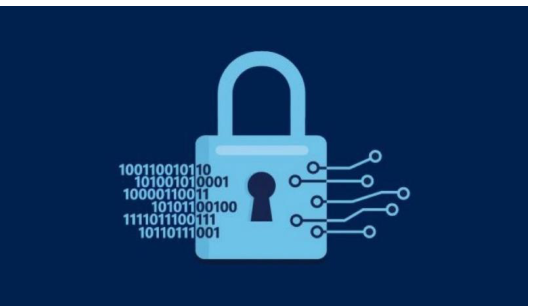
\includegraphics[width=58.38mm,height=84.05mm]{images/llm/page_001_img_01.png}%
\end{textblock*}

% deskripsi: Ilustrasi visual enkripsi data berupa label 'data encryption' di atas keyboard komputer
% bbox normalisasi: [0.0000, 0.6500, 0.2670, 0.9990]
\begin{textblock*}{56.07mm}(0.00mm,193.05mm)
\noindent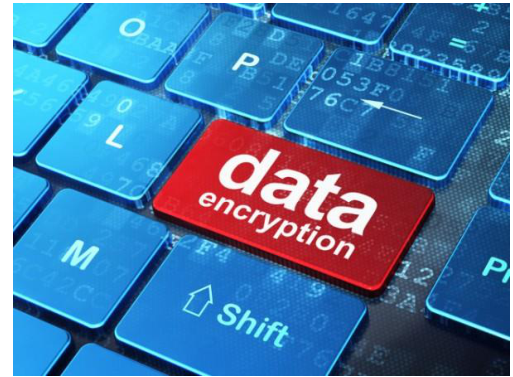
\includegraphics[width=56.07mm,height=103.65mm]{images/llm/page_001_img_02.png}%
\end{textblock*}

\newpage

% --- unit llm 2 ---
% === Halaman 2 (llm) ===

\begin{itemize}
    \item Misalkan Alice dan Bob saling berkomunikasi dengan berkirim pesan:
    \begin{itemize}
        \item via surat menyurat,
        \item via telepon
        \item via email
        \item via SMS
        \item dll
    \end{itemize}
    menggunakan saluran komunikasi publik (pos, telepon, jaringan seluler, internet)
\end{itemize}
\vspace{10mm}

\vspace{74.25mm}

% deskripsi: Ilustrasi komunikasi antara Alice dan Bob dengan tanda panah yang menunjukkan pengiriman pesan dari Alice ke Bob.
% bbox normalisasi: [0.1850, 0.6300, 0.8300, 0.8800]
\begin{textblock*}{135.45mm}(38.85mm,187.11mm)
\noindent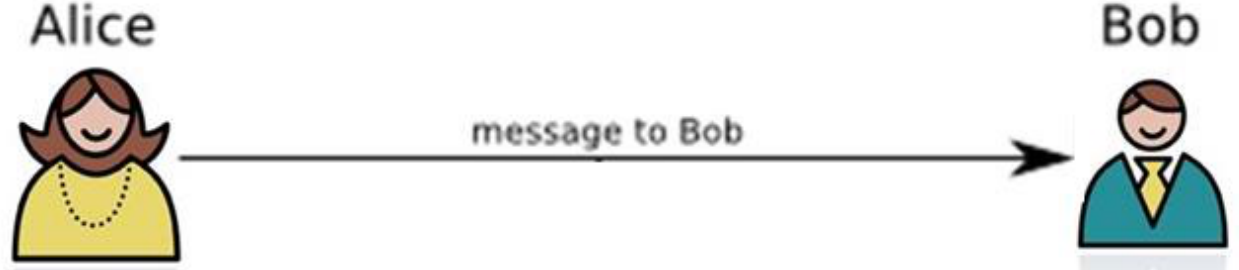
\includegraphics[width=135.45mm,height=74.25mm]{images/llm/page_002_img_01.png}%
\end{textblock*}

\newpage

% --- unit llm 3 ---
% === Halaman 3 (llm) ===

\begin{itemize}
  \item FYI, Alice dan Bob di dalam dunia nyata bisa berupa
  \begin{itemize}
    \item Alice dan Bob adalah manusia dalam arti sesungguhnya
    \item manusia dengan mesin (misalnya mesin penjawab telepon)
    \item mesin dengan mesin (misalnya komputer \textit{client} dengan komputer \textit{server})
    \item web browser dengan sistem server di dalam jaringan komputer
    \item online banking client/server
    \item DNS server, router, mesin penjawab telepon, dsb
  \end{itemize}
\end{itemize}
\vspace{10mm}

\vspace{99.20mm}

% deskripsi: Diagram komunikasi sederhana antara Alice dan Bob yang direpresentasikan sebagai komputer dan manusia, dengan panah yang menunjukkan pengiriman pesan ('message to Bob').
% bbox normalisasi: [0.2070, 0.5460, 0.6950, 0.8800]
\begin{textblock*}{102.48mm}(43.47mm,162.16mm)
\noindent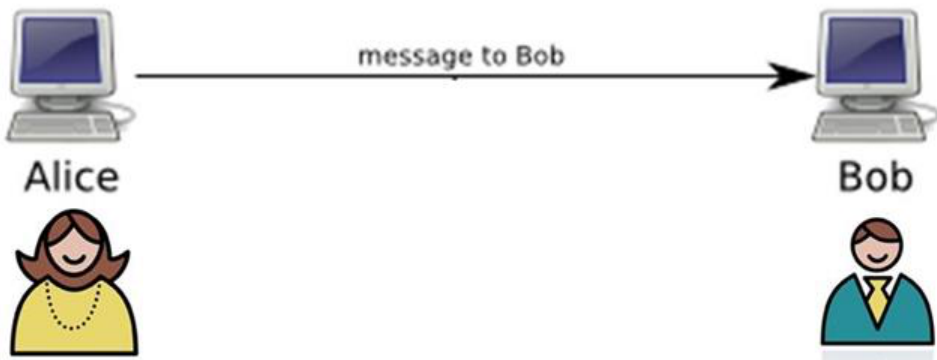
\includegraphics[width=102.48mm,height=99.20mm]{images/llm/page_003_img_01.png}%
\end{textblock*}

\newpage

% --- unit llm 4 ---
% === Halaman 4 (llm) ===

% (tidak ada teks dari model)

% deskripsi: Ilustrasi konsep interaksi antara manusia dan mesin, menampilkan seorang wanita dengan label 'HUMAN' dan sebuah perangkat elektronik dengan label 'MACHINE', keduanya dikelilingi oleh pola titik-garis yang menyerupai jaringan saraf atau pengenalan pola.
% bbox normalisasi: [0.0620, 0.2100, 0.9580, 0.7430]
\begin{textblock*}{188.16mm}(13.02mm,62.37mm)
\noindent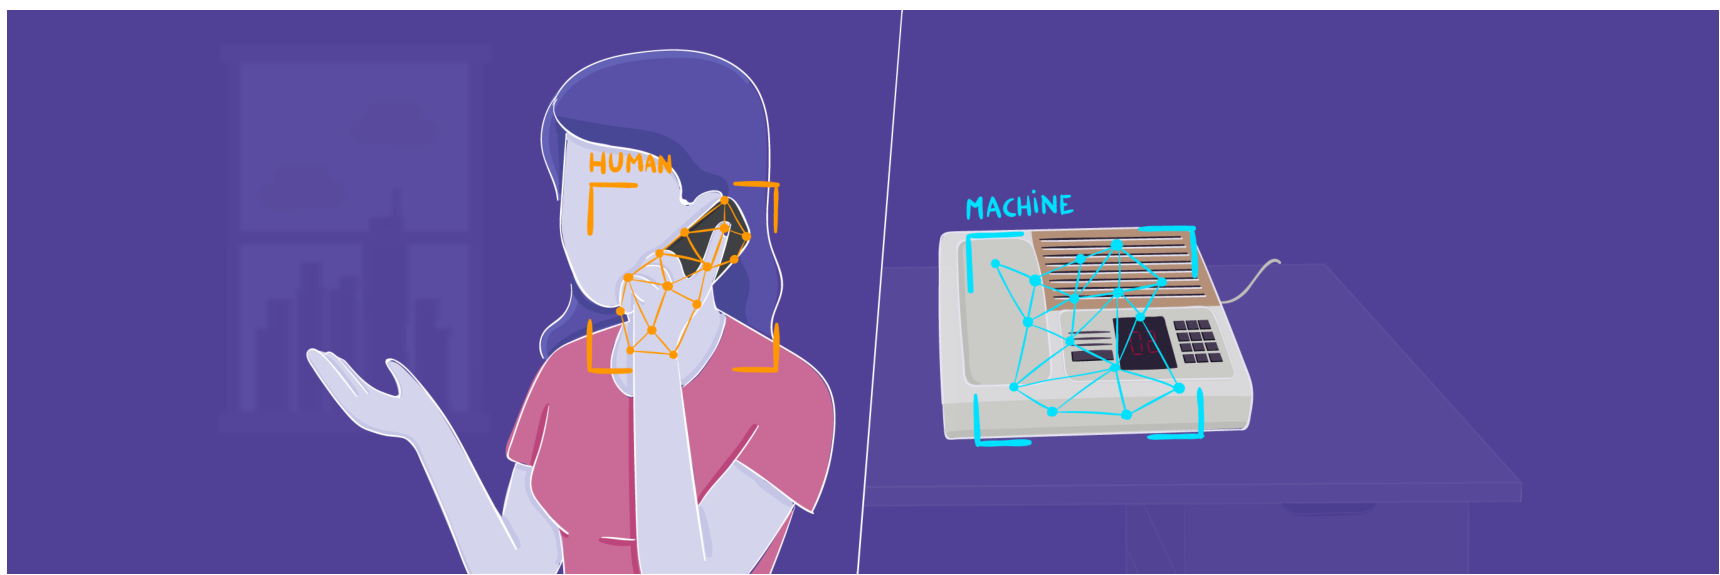
\includegraphics[width=188.16mm,height=158.30mm]{images/llm/page_004_img_01.png}%
\end{textblock*}

\newpage

% --- unit llm 5 ---
% === Halaman 5 (llm) ===

\vspace{103.65mm}

Client
\vspace{50mm}
Browser

% deskripsi: Diagram yang mengilustrasikan siklus permintaan dan tanggapan HTTP antara Client (Browser) dan Server, menunjukkan panah aliran 'HTTP Request' dari client ke server dan 'HTTP Response' dari server kembali ke client.
% bbox normalisasi: [0.2520, 0.2710, 0.6810, 0.6200]
\begin{textblock*}{90.09mm}(52.92mm,80.49mm)
\noindent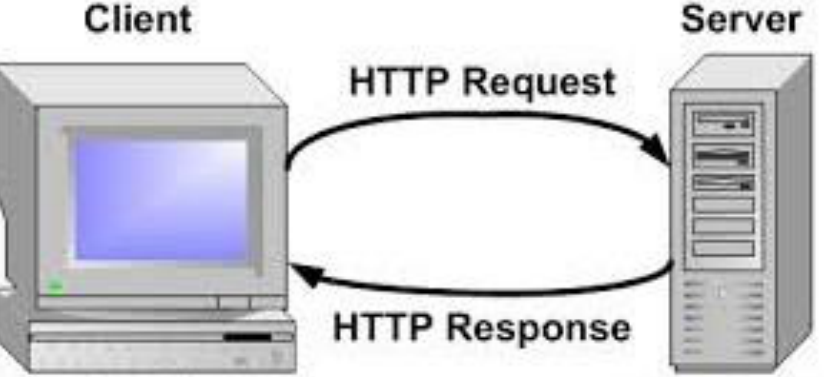
\includegraphics[width=90.09mm,height=103.65mm]{images/llm/page_005_img_01.png}%
\end{textblock*}

\newpage

% --- unit llm 6 ---
% === Halaman 6 (llm) ===

\begin{itemize}
    \item \textbf{Case 1}: Bagaimana Alice memastikan pesan-pesannya tidak dapat dibaca oleh penyadap (\textit{eavesdropper}) yang menguping komunikasinya dengan Bob?
\end{itemize}

\vspace{40mm}

$\rightarrow$ masalah kerahasiaan pesan (\textit{confidentiality})

% deskripsi: Diagram ilustrasi komunikasi antara Alice dan Bob yang disadap oleh Eve (eavesdropper), menunjukkan aliran pesan dari Alice ke Bob dengan panah yang bercabang menuju Eve.
% bbox normalisasi: [0.2200, 0.3300, 0.7300, 0.7200]
\begin{textblock*}{107.10mm}(46.20mm,98.01mm)
\noindent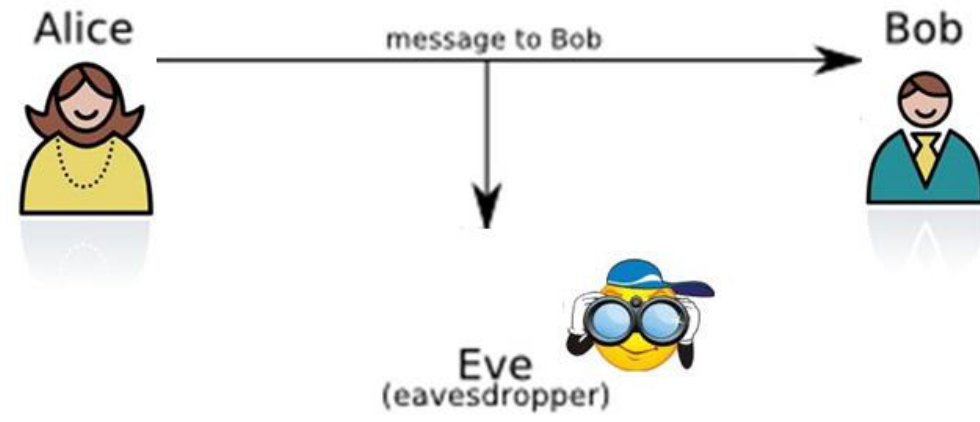
\includegraphics[width=107.10mm,height=115.83mm]{images/llm/page_006_img_01.png}%
\end{textblock*}

\newpage

% --- unit llm 7 ---
% === Halaman 7 (llm) ===

\begin{itemize}
  \item \textbf{Case 2:} Bagaimana cara Bob memastikan bahwa pesan tersebut dari Alice dan bukan dari Carol (yang menyamar menjadi Alice)?
\end{itemize}

\vspace{20mm}

\textcolor{red}{Benarkah ini pesan dari Alice?}

\vspace{40mm}

$\rightarrow$ masalah otentikasi (\textit{authentication}) pengirim atau penerima pesan

% deskripsi: Ilustrasi komunikasi pesan antara Alice dan Bob dengan tanda panah yang menunjukkan arah pengiriman pesan.
% bbox normalisasi: [0.2040, 0.3850, 0.7430, 0.6110]
\begin{textblock*}{113.19mm}(42.84mm,114.34mm)
\noindent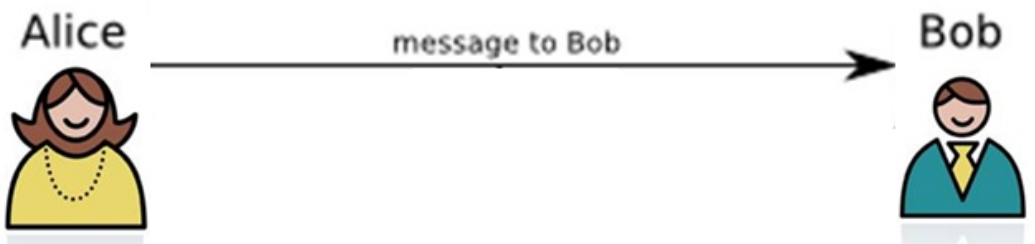
\includegraphics[width=113.19mm,height=67.12mm]{images/llm/page_007_img_01.png}%
\end{textblock*}

\newpage

% --- unit llm 8 ---
% === Halaman 8 (llm) ===

\begin{itemize}
    \item \textbf{Case 3}: Bagaimana cara Bob memastikan bahwa pesan dari Alice masih utuh, asli, tidak diubah, atau dimanipulasi selama komunikasi,
\end{itemize}

\vspace{40mm}

$\rightarrow$ masalah keutuhan (\textit{integrity}) pesan?

% deskripsi: Ilustrasi proses komunikasi dari Alice ke Bob dengan teks pertanyaan 'Sudah diubah atau masih asli kah pesan dari Alice ini?' yang menunjukkan konsep integritas data.
% bbox normalisasi: [0.1900, 0.2900, 0.9400, 0.6800]
\begin{textblock*}{157.50mm}(39.90mm,86.13mm)
\noindent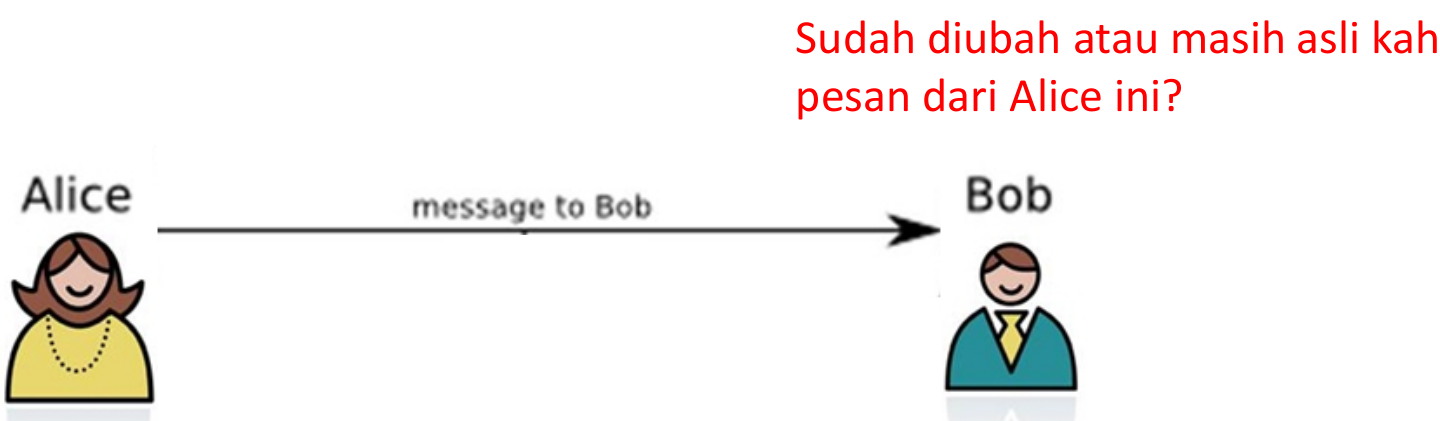
\includegraphics[width=157.50mm,height=115.83mm]{images/llm/page_008_img_01.png}%
\end{textblock*}

\newpage

% --- unit llm 9 ---
% === Halaman 9 (llm) ===

\begin{itemize}
    \item \textbf{Case 4:} Bagaimana Bob melakukan anti-sangkalan apabila Alice menyangkal telah mengirim pesan kepada Bob?
\end{itemize}

\textcolor{red}{Swer, saya nggak pernah kirim pesan ini kepadamu, Bob!} \hfill \textcolor{red}{Hmmmmm....}

\vspace{30mm}

$\rightarrow$ masalah nir-penyangkalan (non-repudiation)

% deskripsi: Diagram ilustrasi pengiriman pesan dari Alice ke Bob yang menggambarkan masalah non-repudiation, dengan panah menunjukkan aliran pesan dan karakter Alice dan Bob.
% bbox normalisasi: [0.1800, 0.4500, 0.7600, 0.7100]
\begin{textblock*}{121.80mm}(37.80mm,133.65mm)
\noindent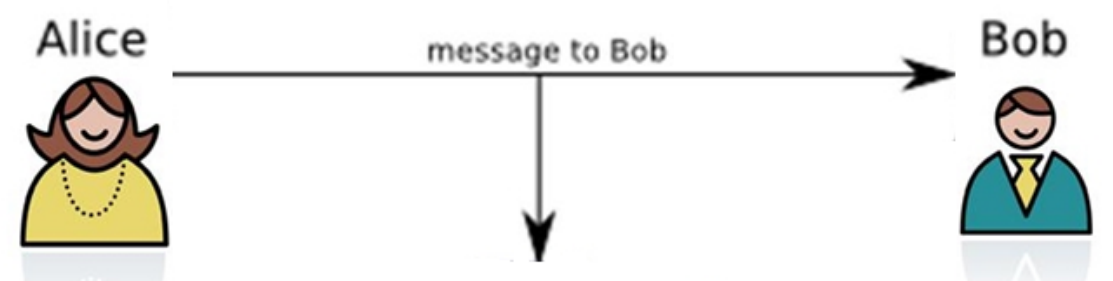
\includegraphics[width=121.80mm,height=77.22mm]{images/llm/page_009_img_01.png}%
\end{textblock*}

\newpage

% --- unit llm 10 ---
% === Halaman 10 (llm) ===

\begin{itemize}
    \item Keempat masalah tersebut:
    \begin{itemize}
        \item \textit{confidentiality},
        \item \textit{authentication},
        \item \textit{data integrity},
        \item \textit{non-repudiation}
    \end{itemize}
\end{itemize}

solusinya adalah menggunakan KRIPTOGRAFI

\newpage

% --- unit llm 11 ---
% === Halaman 11 (llm) ===

\section*{Kriptografi}

\vspace{114.05mm}

\begin{itemize}
    \item Kata \textit{cryptography} berasal dari bahasa Yunani:
    \begin{itemize}
        \item \textcolor{red}{crypt\acute{o}s} (secret or hidden)
        \item \textcolor{red}{gr\acute{a}phein} (writing)
    \end{itemize}
    Artinya "secret writing or "hidden writing"

    \vspace{20mm}
    \item \textbf{Kriptografi}: ilmu dan seni untuk menjaga keamanan pesan. (Schneier, 1996)
\end{itemize}

\noindent Definisi lainnya:\n\textbf{Kriptografi} adalah ilmu yang mempelajari teknik-teknik matematika yang berhubungan dengan aspek keamanan informasi seperti kerahasiaan, integritas data, serta otentikasi (Menez, 1996)

% deskripsi: Ilustrasi berupa kumpulan kode hexadecimal dan teks keamanan dalam lingkaran biru di atas latar belakang bertekstur digital
% bbox normalisasi: [0.6140, 0.1440, 0.9850, 0.5280]
\begin{textblock*}{77.91mm}(128.94mm,42.77mm)
\noindent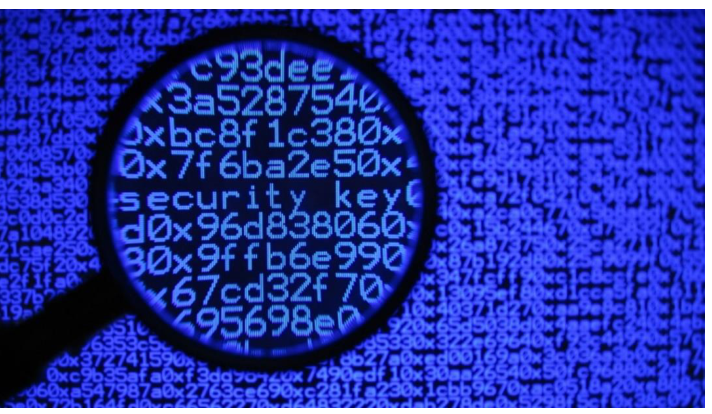
\includegraphics[width=77.91mm,height=114.05mm]{images/llm/page_011_img_01.png}%
\end{textblock*}

\newpage

% --- unit llm 12 ---
% === Halaman 12 (llm) ===

“Aman” artinya:

\vspace{95.04mm}

\begin{enumerate}
  \item \textbf{Terjaga kerahasiaannya (confidentiality)}
  \vspace{50mm}
  \item \textbf{Terjaga keasliannya (data integrity)}
  \vspace{50mm}
\end{enumerate}

% deskripsi: Dua kotak teks yang membandingkan teks asli (plainteks) dengan teks terenkripsi (cipherteks) untuk menjelaskan konsep kerahasiaan data.
% bbox normalisasi: [0.0700, 0.2000, 0.5600, 0.4700]
\begin{textblock*}{102.90mm}(14.70mm,59.40mm)
\noindent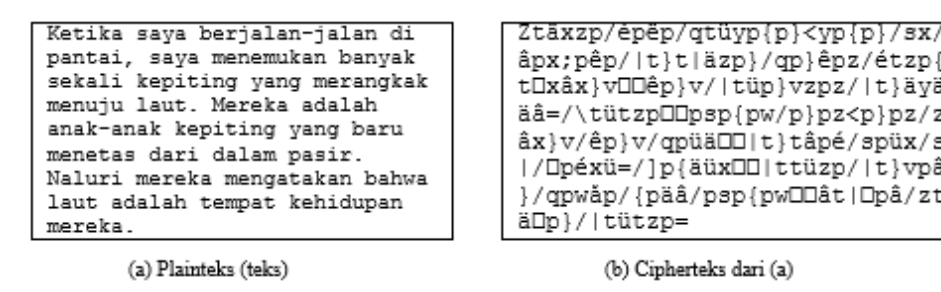
\includegraphics[width=102.90mm,height=80.19mm]{images/llm/page_012_img_01.png}%
\end{textblock*}

% deskripsi: Perbandingan dua kotak teks suhu (33 derajat vs 32 derajat) dan dua foto bebek yang hampir identik untuk mengilustrasikan perubahan data (integritas data).
% bbox normalisasi: [0.0900, 0.6300, 0.9600, 0.9500]
\begin{textblock*}{182.70mm}(18.90mm,187.11mm)
\noindent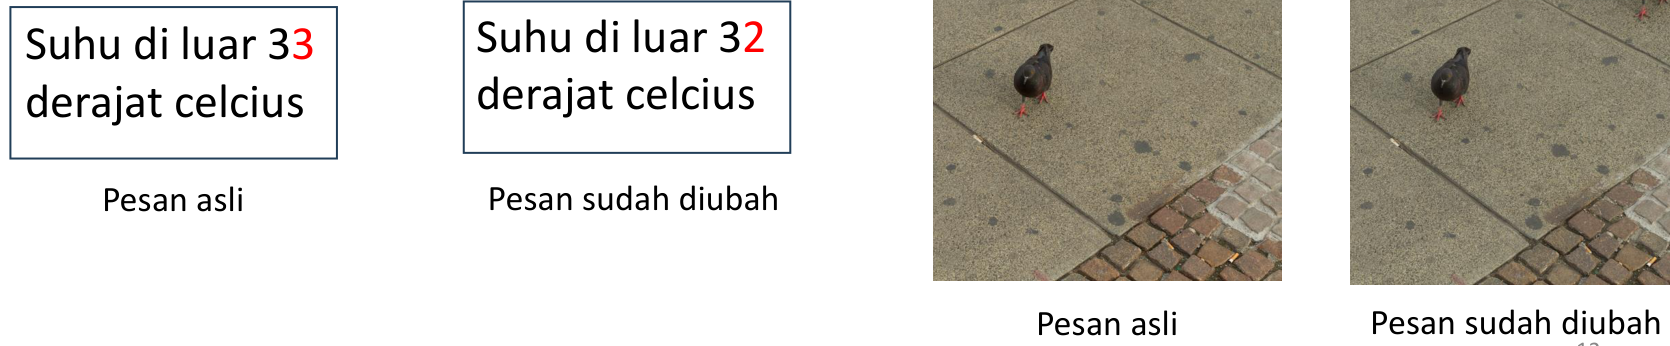
\includegraphics[width=182.70mm,height=95.04mm]{images/llm/page_012_img_02.png}%
\end{textblock*}

\newpage

% --- unit llm 13 ---
% === Halaman 13 (llm) ===

\vspace{136.62mm}

3. Yakin pengirim pesan adalah asli (authentication), bukan pihak ketiga yang menyerupai.\vspace{50mm}
\begin{center}
Dia mengklaim bahwa dia adalah $A$
\end{center}
\vspace{50mm}
4. Pengirim pesan tidak dapat menyangkal (non repudiation) telah mengirim pesan.

% deskripsi: Ilustrasi konsep autentikasi yang menunjukkan dua pihak A dan B dengan pihak ketiga di tengah yang mencoba menyerupai A.
% bbox normalisasi: [0.0380, 0.3400, 0.3800, 0.7400]
\begin{textblock*}{71.82mm}(7.98mm,100.98mm)
\noindent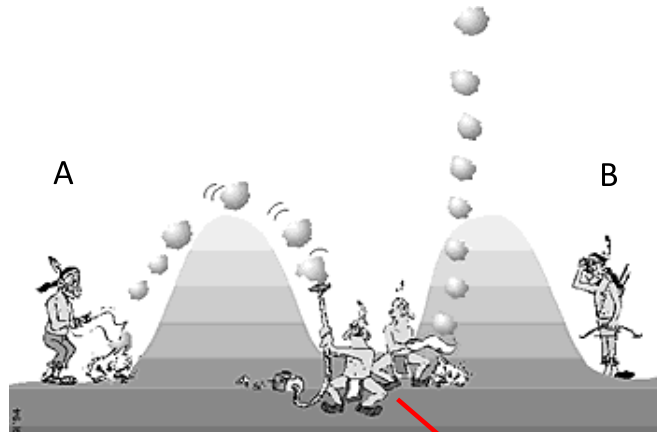
\includegraphics[width=71.82mm,height=118.80mm]{images/llm/page_013_img_01.png}%
\end{textblock*}

% deskripsi: Diagram konsep Non-Repudiation yang menunjukkan proses transfer dana dan penyangkalan pengiriman pesan.
% bbox normalisasi: [0.5450, 0.3600, 0.8970, 0.8200]
\begin{textblock*}{73.92mm}(114.45mm,106.92mm)
\noindent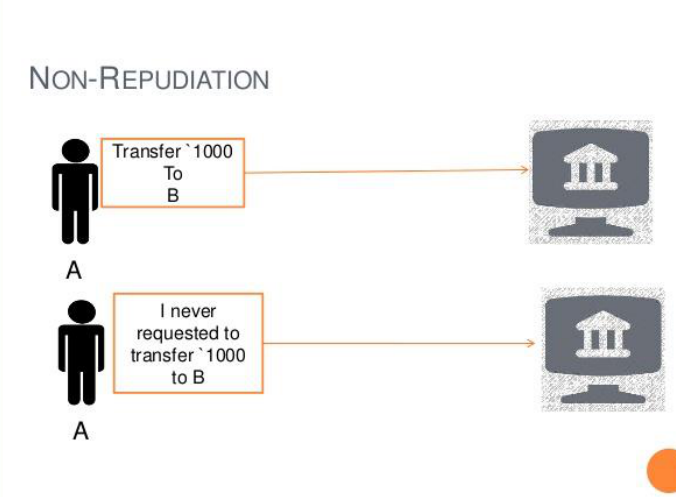
\includegraphics[width=73.92mm,height=136.62mm]{images/llm/page_013_img_02.png}%
\end{textblock*}

\newpage

% --- unit llm 14 ---
% === Halaman 14 (llm) ===

\section*{Empat Layanan Kriptografi}

\vspace{72.17mm}

\begin{enumerate}
    \item Kerahasiaan pesan (\textit{Confidentiality/privacy/secrecy})
    \vspace{20mm}
    \item Keaslian pesan (\textit{Data integrity})
    \vspace{15mm}
    \item Keaslian pengirim dan penerima pesan (\textit{Authentication})
    \vspace{15mm}
    \item Anti penyangkalan (\textit{Non-repudiation})
\end{enumerate}

\vspace{49.30mm}

% deskripsi: Stempel merah bertuliskan 'PRIVATE & CONFIDENTIAL' sebagai representasi kerahasiaan.
% bbox normalisasi: [0.7280, 0.1460, 0.9300, 0.3110]
\begin{textblock*}{42.42mm}(152.88mm,43.36mm)
\noindent
\includegraphics[width=42.42mm,height=49.01mm]{images/llm/page_014_img_01.png}%
\end{textblock*}

% deskripsi: Ilustrasi teks 'Data Integrity' di atas latar belakang kode biner untuk merepresentasikan integritas data.
% bbox normalisasi: [0.4740, 0.2670, 0.6970, 0.5100]
\begin{textblock*}{46.83mm}(99.54mm,79.30mm)
\noindent
\includegraphics[width=46.83mm,height=72.17mm]{images/llm/page_014_img_02.png}%
\end{textblock*}

% deskripsi: Ilustrasi proses autentikasi melalui smartphone dengan pertanyaan 'Is this you?' dan tombol akses.
% bbox normalisasi: [0.4810, 0.5240, 0.7450, 0.7550]
\begin{textblock*}{55.44mm}(101.01mm,155.63mm)
\noindent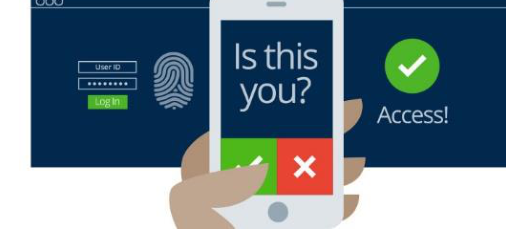
\includegraphics[width=55.44mm,height=68.61mm]{images/llm/page_014_img_03.png}%
\end{textblock*}

% deskripsi: Diagram konsep non-repudiation yang menunjukkan pengiriman dokumen dari individu ke bank dengan bukti pengiriman.
% bbox normalisasi: [0.5820, 0.7720, 0.7410, 0.9380]
\begin{textblock*}{33.39mm}(122.22mm,229.28mm)
\noindent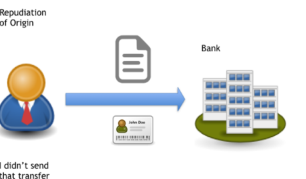
\includegraphics[width=33.39mm,height=49.30mm]{images/llm/page_014_img_04.png}%
\end{textblock*}

\newpage

% --- unit llm 15 ---
% === Halaman 15 (llm) ===

"Cryptography lies at the heart of all cybersecuriry technologies, and understanding the role it plays is vital to understanding how to secure cyberspace" (Keith M. Martin)

\textcolor{red}{(Kriptografi merupakan inti dari semua teknologi keamanan siber, dan memahami peran yang dimainkannya sangat penting untuk memahami cara mengamankan ruang siber)}

\vspace{10mm}

Kriptografer masih menjadi sosok yang langka di Indonesia. Namun, bidang ini sangat penting untuk segera ditumbuhkan

\newpage

% --- unit llm 16 ---
% === Halaman 16 (llm) ===

\section*{Masih ingat dengan kasus-kasus ini?}

\vspace{117.61mm}

\begin{itemize}
    \item \textbf{Wikileaks}
    \begin{itemize}
        \item pembocoran dokumen Perang Afghanistan (Juli, 2010)
        \item Pembocoran 400.000 dokumen Perang Irak (Oktober 2010)
        \item Pembocoran kawat diplomatik Amerika Serikat (November 2010)
        \item dll
    \end{itemize}
\end{itemize}

\vspace{20mm}

\textcolor{red}{Julian Assange}, salah satu pendiri situs WikiLeaks.

% deskripsi: Foto Julian Assange dengan latar belakang logo WikiLeaks dan peta dunia
% bbox normalisasi: [0.5870, 0.2060, 0.9840, 0.6020]
\begin{textblock*}{83.37mm}(123.27mm,61.18mm)
\noindent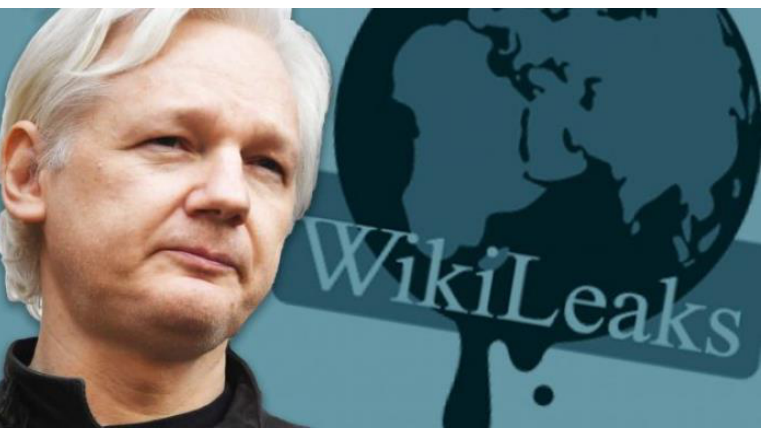
\includegraphics[width=83.37mm,height=117.61mm]{images/llm/page_016_img_01.png}%
\end{textblock*}

% deskripsi: Kliping berita theguardian tentang WikiLeaks dan foto Julian Assange
% bbox normalisasi: [0.1860, 0.6760, 0.4030, 0.9880]
\begin{textblock*}{45.57mm}(39.06mm,200.77mm)
\noindent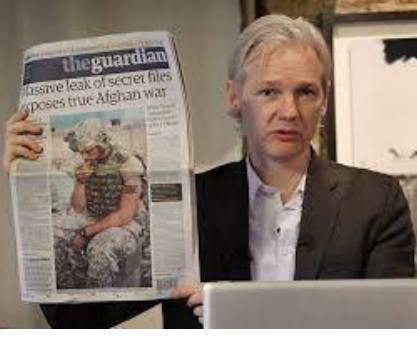
\includegraphics[width=45.57mm,height=92.66mm]{images/llm/page_016_img_02.png}%
\end{textblock*}

% deskripsi: Sampul majalah TIME yang menampilkan Julian Assange dengan judul 'Do You Want to Know a Secret?'
% bbox normalisasi: [0.4310, 0.6440, 0.5760, 0.9880]
\begin{textblock*}{30.45mm}(90.51mm,191.27mm)
\noindent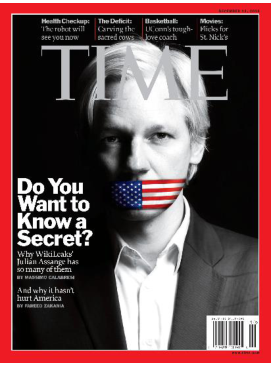
\includegraphics[width=30.45mm,height=102.17mm]{images/llm/page_016_img_03.png}%
\end{textblock*}

% deskripsi: Sampul buku atau artikel mengenai Indonesia, WikiLeaks, dan Julian Assange
% bbox normalisasi: [0.7480, 0.6810, 0.8640, 0.9880]
\begin{textblock*}{24.36mm}(157.08mm,202.26mm)
\noindent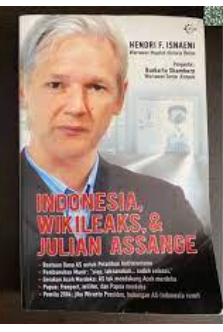
\includegraphics[width=24.36mm,height=91.18mm]{images/llm/page_016_img_04.png}%
\end{textblock*}

\newpage

% --- unit llm 17 ---
% === Halaman 17 (llm) ===

\begin{itemize}
  \item Penyadapan di Kedubes RI di luar negeri
\end{itemize}

\vspace{10mm}

\textbf{Menlu: Penyadapan KBRI di Myanmar Langgar Konvensi Wina}

- detikNews

Rabu, 14 Jul 2004 14:47 WIB

\textbf{Banten} - Menteri Luar Negeri Hasan Wirajuda menyesalkan terjadinya indikasi penyadapan kantor Kedutaan Besar RI di Yangoon. Penyadapan dinilai melanggar konvensi Wina. Kedubes Myanmar hingga kini masih berkelit. "Ada indikasi kuat mengarah kesana. Itu berdasarkan temuan tim dan hasil pemeriksaan. Atas peristiwa ini, kita sampaikan keprihatinan yang mendalam dan keras bahwa ini terjadi antar sesama anggota Asean dan jelas melanggar konvensi Wina. Dalam konvensi itu dilarang mengganggu fasilitas kedutaan karena itu menyangkut masalah kerahasiaan," Hal ini disampaikan Menteri Luar Negeri Hasan Wirajuda usai mendampingi Presiden Megawati Soekarnoputri pada peringatan Dasawarsa Konprensi Internasional Kependudukan dan Pembangunan di Kabupaten Pandeglang, Provinsi Banten, Rabu (14/7/2004).Menurut

% deskripsi: Screenshot artikel berita dari situs detiknews mengenai penyadapan KBRI di Myanmar
% bbox normalisasi: [0.1800, 0.1800, 0.7500, 0.9100]
\begin{textblock*}{119.70mm}(37.80mm,53.46mm)
\noindent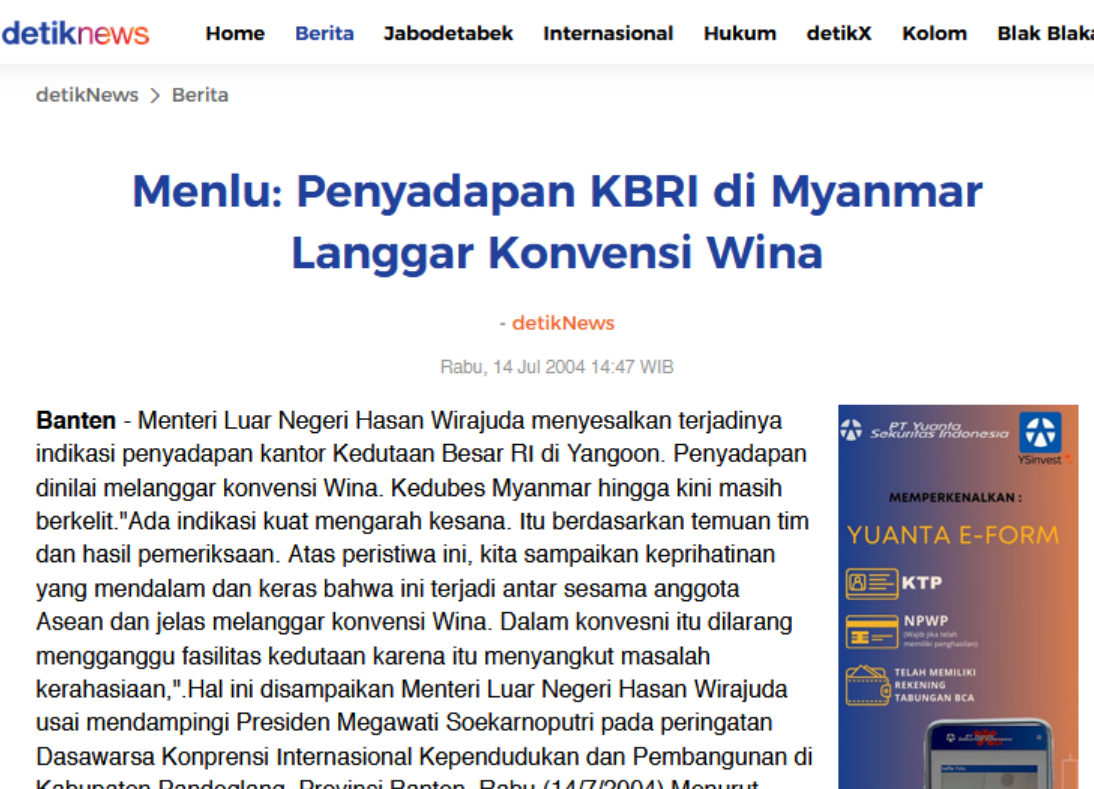
\includegraphics[width=119.70mm,height=216.81mm]{images/llm/page_017_img_01.png}%
\end{textblock*}

\newpage

% --- unit llm 18 ---
% === Halaman 18 (llm) ===

\begin{itemize}
  \item Penyadapan telepon Presiden SBY oleh Pemerintah Australia
\end{itemize}

\vspace{10mm}

Jakarta, Setkab -Pemerintah Indonesia akan memanggil Duta Besar RI dari Australia menyusul dugaan penyadapan telepon Presiden Yudhoyono oleh pemerintah Australia. Menteri Luar Negeri Marty Natalegawa menyampaikan hal ini dalam jumpa pers mendadak di kantor Kementerian Luar Negeri pada Senin (18/11).

"Indonesia akan memanggil pulang Dubes di Canberra untuk konsultasi. Ini tidak bisa dianggap ringan. Ini menunjukkan sikap tegas dan terukur," kata Menlu Marty.

Marty menambahkan mengatakan tindakan itu melukai hubungan kedua negara. "Australia telah melanggar privasi individual, hak asasi manusia dan melukai hubungan Australia-Indonesia," katanya.

% deskripsi: Foto Menteri Luar Negeri Marty Natalegawa sedang memberikan keterangan pers di hadapan awak media.
% bbox normalisasi: [0.1720, 0.2010, 0.5700, 0.6030]
\begin{textblock*}{83.58mm}(36.12mm,59.70mm)
\noindent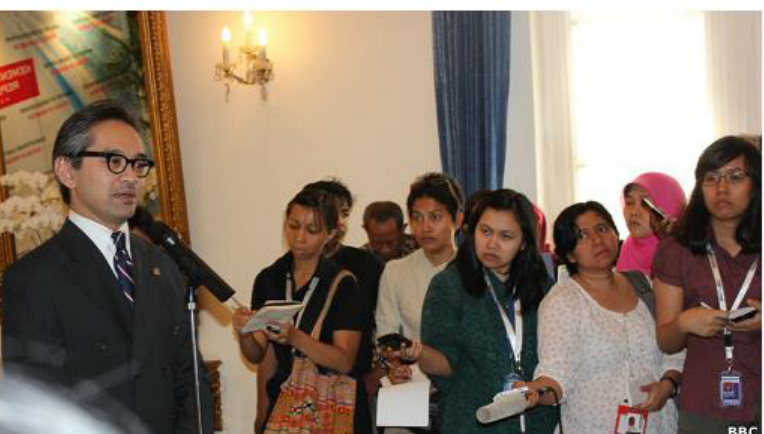
\includegraphics[width=83.58mm,height=119.39mm]{images/llm/page_018_img_01.png}%
\end{textblock*}

\newpage

% --- unit llm 19 ---
% === Halaman 19 (llm) ===

\section*{Kebocoran data BPJS}

\vspace{50mm}

\begin{itemize}
    \item \textbf{KEBOCORAN DATA PRIBADI YANG TERUS BERULANG}
    \item DATA BPJS KESEHATAN BOCOR
    \begin{itemize}
        \item 279 juta data pengguna diperjualbelikan (Mei 2021)
        \item NIK nama, alamat, No phone, e-mail, foto
        \item Dijual di Raid Forums
        \item Harga jual 0.15 BTC (Rp 70-80 juta)
    \end{itemize}
    \item \textbf{Langkah pemerintah}
    \begin{itemize}
        \item Akses unduhan ditutup
        \item Bloker situs Raid Forums
        \item Investigasi
    \end{itemize}
    \item \textbf{KEBOCORAN DATA PERNAH TERJADI}
    \begin{itemize}
        \item Kasus 2020
        \begin{itemize}
            \item 91 juta data pengguna \& 7 juta data merchant (Tokopedia)
            \item 2,3 juta data pemilih Pemilu 2014 (KPU)
            \item 250 ribu data pasien Covid-19
        \end{itemize}
    \end{itemize}
    \item \textbf{Pentingnya regulasi}
    \begin{itemize}
        \item Masyarakat berhak:
        \begin{itemize}
            \item Tahu tujuan penggunaan data
            \item Hapus data ke pengelola
        \end{itemize}
        \item Pengelola wajib mitigasi kebocoran
        \item Sanksi/denda jika bocor
        \end{itemize}
    \end{itemize}
\end{itemize}

% deskripsi: Screenshot forum gelap yang menunjukkan postingan penjualan data warga negara Indonesia (NIK, KTP, Phone, dll) oleh pengguna bernama 'kotz'.
% bbox normalisasi: [0.0700, 0.1800, 0.5770, 0.7210]
\begin{textblock*}{106.47mm}(14.70mm,53.46mm)
\noindent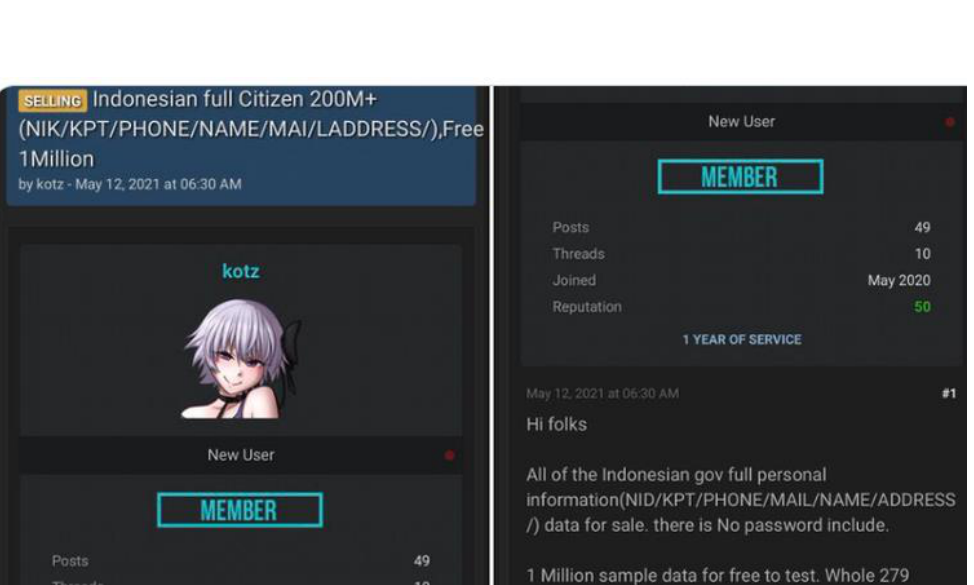
\includegraphics[width=106.47mm,height=160.68mm]{images/llm/page_019_img_01.png}%
\end{textblock*}

% deskripsi: Ilustrasi visual berupa tumpukan kertas dokumen yang diberi cap 'TOP SECRET' sebagai representasi kebocoran data.
% bbox normalisasi: [0.6140, 0.3280, 0.7600, 0.6560]
\begin{textblock*}{30.66mm}(128.94mm,97.42mm)
\noindent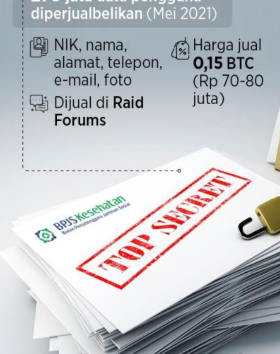
\includegraphics[width=30.66mm,height=97.42mm]{images/llm/page_019_img_02.png}%
\end{textblock*}

\newpage

% --- unit llm 20 ---
% === Halaman 20 (llm) ===

\vspace{286.31mm}

\section*{Kebocoran data penguna Tokopedia}

\vspace{10mm}

\vspace{10mm}

% deskripsi: Screenshot cuitan Twitter dari akun Under the Breach yang menginformasikan kebocoran database Tokopedia pada Maret 2020, lengkap dengan cuplikan data yang bocor.
% bbox normalisasi: [0.0970, 0.1830, 0.5410, 0.8860]
\begin{textblock*}{93.24mm}(20.37mm,54.35mm)
\noindent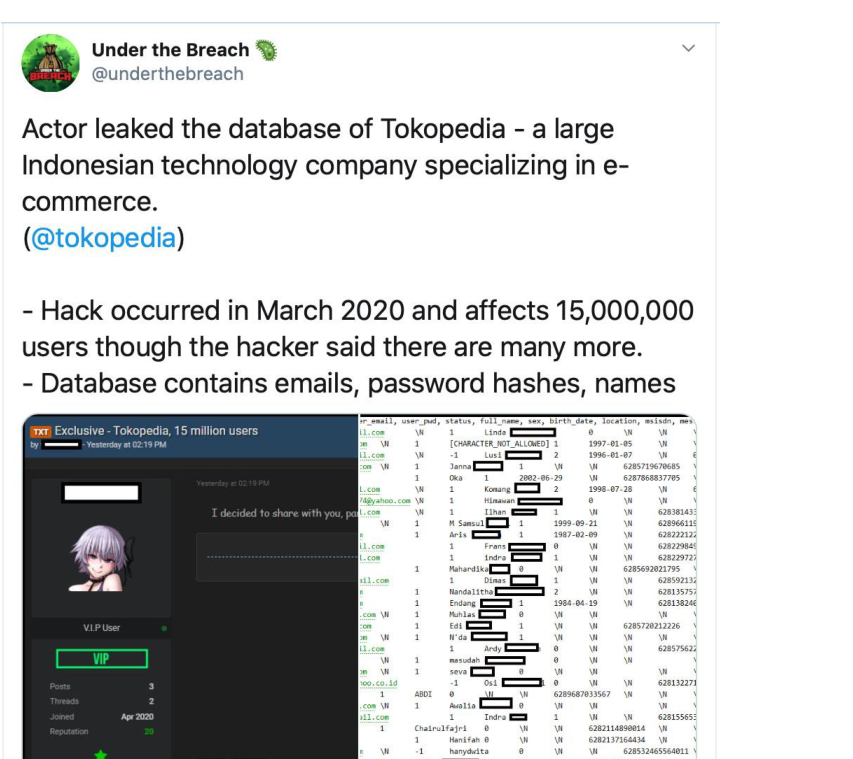
\includegraphics[width=93.24mm,height=208.79mm]{images/llm/page_020_img_01.png}%
\end{textblock*}

% deskripsi: Infografis dari Katadata mengenai pencurian data di e-commerce, merinci kebocoran data Tokopedia (2020) dan Bukalapak (2019) termasuk jumlah data dan harga jualnya.
% bbox normalisasi: [0.6100, 0.0000, 0.9030, 0.9640]
\begin{textblock*}{61.53mm}(128.10mm,0.00mm)
\noindent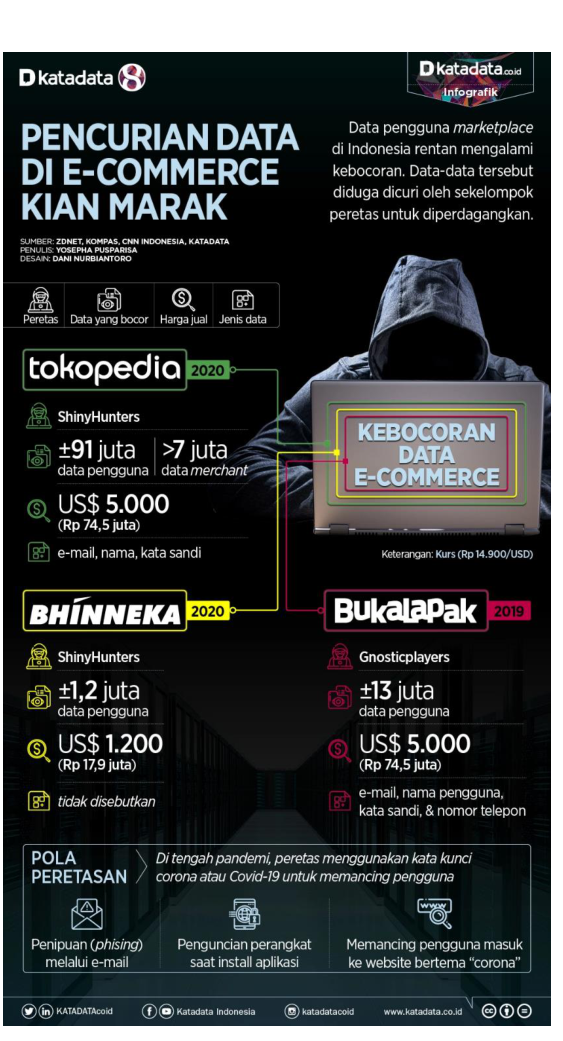
\includegraphics[width=61.53mm,height=286.31mm]{images/llm/page_020_img_02.png}%
\end{textblock*}

\newpage

% --- unit llm 21 ---
% === Halaman 21 (llm) ===

\begin{itemize}
    \item Dugaan kebocoran data pemilih Pemilu 2014, kebocoran sertifikat vaksin Jokowi
\end{itemize}

\vspace{10mm}

% deskripsi: Tangkapan layar berita Kompas.com mengenai kebocoran sertifikat vaksin Jokowi.
% bbox normalisasi: [0.1200, 0.2700, 0.5700, 0.9500]
\begin{textblock*}{94.50mm}(25.20mm,80.19mm)
\noindent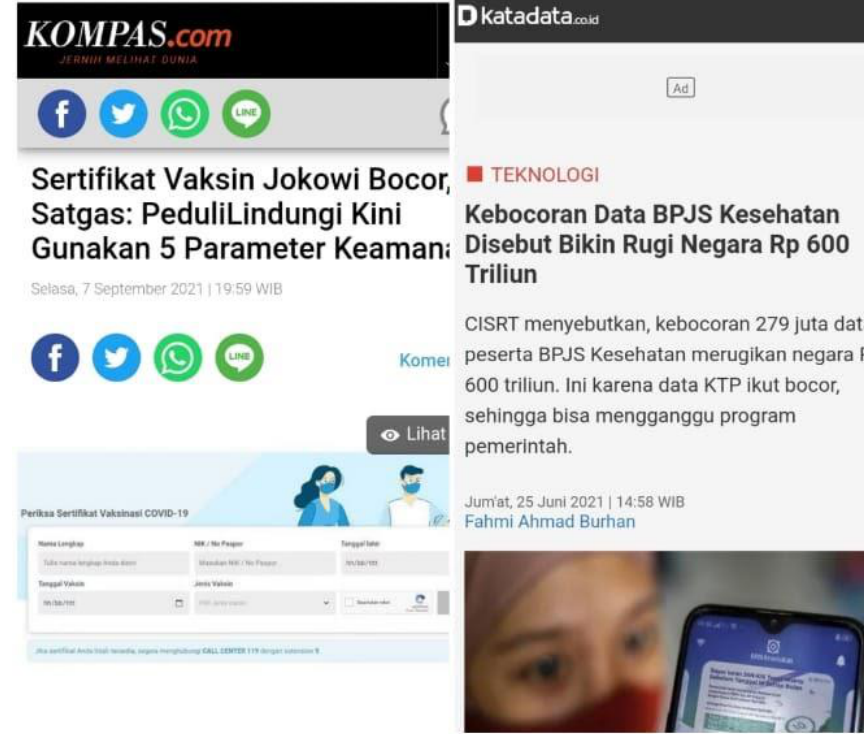
\includegraphics[width=94.50mm,height=201.96mm]{images/llm/page_021_img_01.png}%
\end{textblock*}

% deskripsi: Tangkapan layar berita Katadata mengenai kebocoran data BPJS Kesehatan.
% bbox normalisasi: [0.3500, 0.2600, 0.5800, 0.9500]
\begin{textblock*}{48.30mm}(73.50mm,77.22mm)
\noindent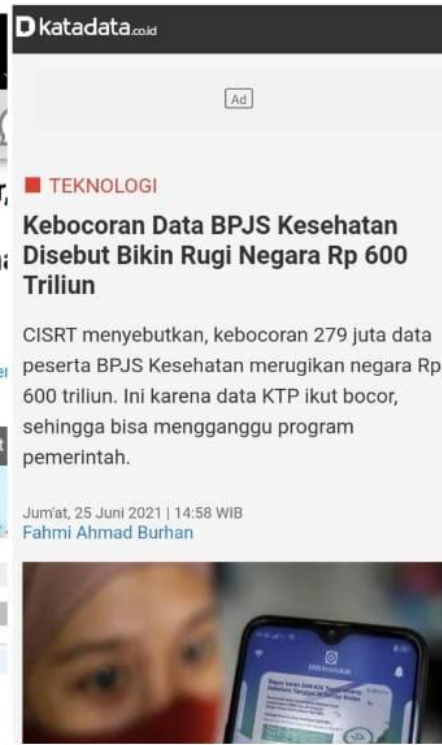
\includegraphics[width=48.30mm,height=204.93mm]{images/llm/page_021_img_02.png}%
\end{textblock*}

% deskripsi: Tangkapan layar berita Kompas.com mengenai dugaan kebocoran data pemilih Pemilu 2014.
% bbox normalisasi: [0.5800, 0.2600, 0.8200, 0.9500]
\begin{textblock*}{50.40mm}(121.80mm,77.22mm)
\noindent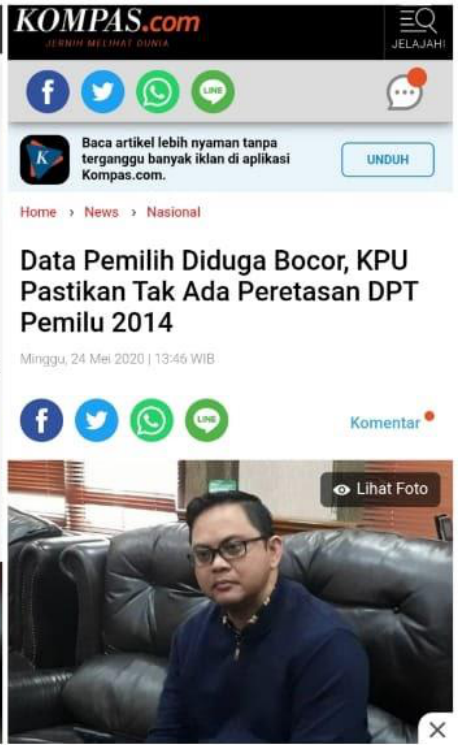
\includegraphics[width=50.40mm,height=204.93mm]{images/llm/page_021_img_03.png}%
\end{textblock*}

\newpage

% --- unit llm 22 ---
% === Halaman 22 (llm) ===

\begin{itemize}
    \item Kebocoran data di Kemenhan dan Bank BSI
\end{itemize}

\vspace{5mm}

\begin{center}
    \textbf{KEJAHATAN SIBER}\\
    \Huge \textbf{Situs Kementerian Pertahanan Diduga Diretas, Dokumen Rahasia Berpotensi Bocor}\\
    Data Kementerian Pertahanan sebesar 1,64 terabita berpotensi bocor setelah situs resmi kementerian itu dibobol peretas.
\end{center}

\vspace{10mm}

\begin{center}
    \huge \textbf{1,5 TB Data Nasabah BSI Dibobol Hacker LockBit 3.0}\\
    \small Taufan Bara Mukti $\square$ Sabtu, 13 Mei 2023 | 12:03 WIB
\end{center}

% deskripsi: Foto gedung Bank Syariah Indonesia (BSI) sebagai ilustrasi berita kebocoran data.
% bbox normalisasi: [0.2070, 0.7030, 0.7200, 1.0000]
\begin{textblock*}{107.73mm}(43.47mm,208.79mm)
\noindent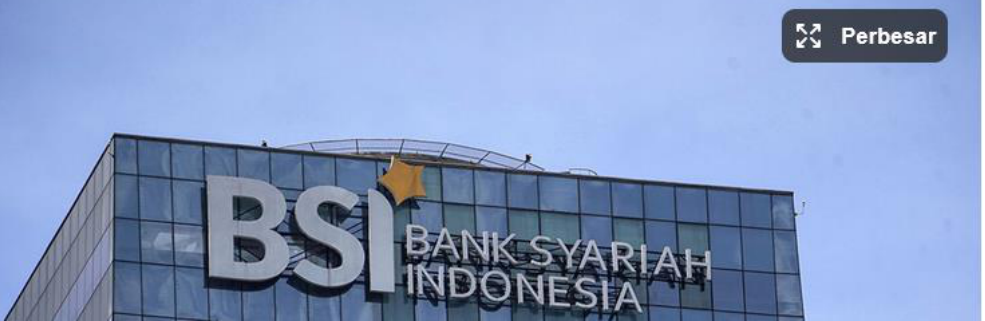
\includegraphics[width=107.73mm,height=88.21mm]{images/llm/page_022_img_01.png}%
\end{textblock*}

\newpage

% --- unit llm 23 ---
% === Halaman 23 (llm) ===

\vspace{212.65mm}

\section*{Deretan Kasus Dugaan Kebocoran Data di RI}

\vspace{80mm}

...dan masih banyak lagi

% deskripsi: Infografis timeline rangkaian kasus dugaan kebocoran data di Indonesia dari tahun 2020 hingga 2022, menampilkan bulan dan jumlah data yang bocor.
% bbox normalisasi: [0.1010, 0.1540, 0.5170, 0.8700]
\begin{textblock*}{87.36mm}(21.21mm,45.74mm)
\noindent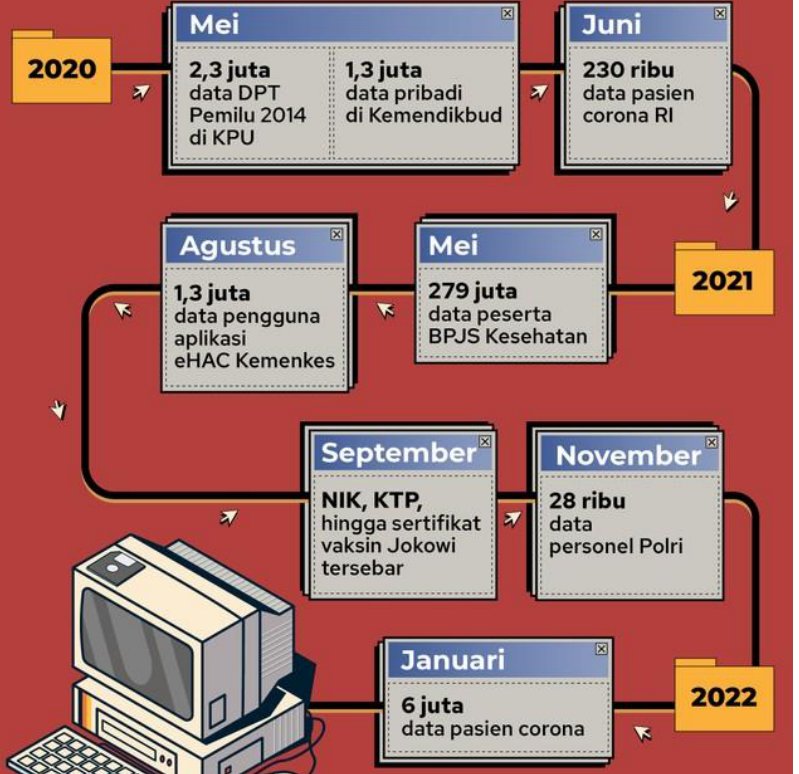
\includegraphics[width=87.36mm,height=212.65mm]{images/llm/page_023_img_01.png}%
\end{textblock*}

\newpage

% --- unit llm 24 ---
% === Halaman 24 (llm) ===

\begin{itemize}
  \item Kasus-kasus seperti:
  \begin{itemize}
    \item kebocoran data,
    \item pencurian data,
    \item pengaksesan data secara ilegal, dll
  \end{itemize}
\end{itemize}

menunjukkan pentingnya \textcolor{red}{kriptografi} menjaga keamanan data dan informasi.

\newpage

% --- unit llm 25 ---
% === Halaman 25 (llm) ===

\section*{Terminologi di dalam Kriptografi}

\begin{enumerate}
    \item \textbf{Pesan}: data atau informasi yang dapat dibaca dan dimengerti maknanya (baik dipersepsi secara visual maupun audial)\
    Nama lain: \textbf{plainteks} (plaintext), \textit{plain-image}, \textit{plain-video}, \textit{plain-video}
\end{enumerate}

Di dalam kriptografi, data dan informasi disebut pesan (\textit{message})

Rupa pesan: teks, gambar, musik, video, tabel, daftar belanja, gambar 3D, sinyal control, dll

\newpage

% --- unit llm 26 ---
% === Halaman 26 (llm) ===

\vspace{117.02mm}

(a) Teks\n\n"Kita semua bersaudara"\n"Hello, world!"\n"Namaku Alice"
\vspace{50mm}
(c) Audio\n\nSumber: http://cloudinary.com

\vspace{86.72mm}

% deskripsi: Foto berbagai macam paprika warna-warni
% bbox normalisasi: [0.0600, 0.1080, 0.9400, 0.5020]
\begin{textblock*}{184.80mm}(12.60mm,32.08mm)
\noindent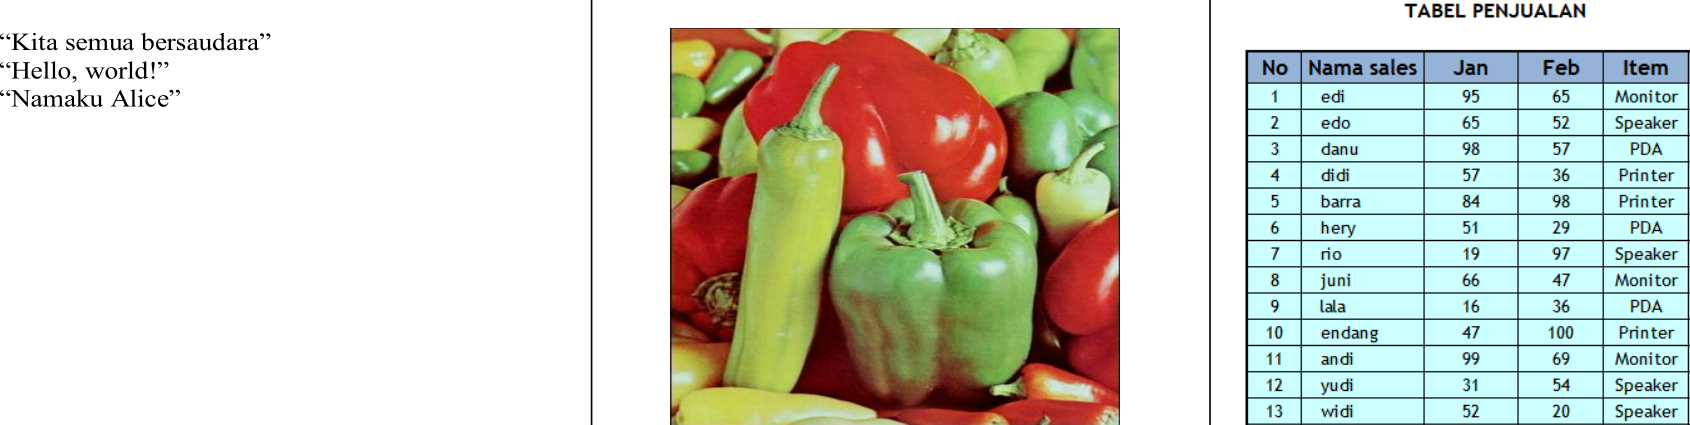
\includegraphics[width=184.80mm,height=117.02mm]{images/llm/page_026_img_01.png}%
\end{textblock*}

% deskripsi: Tabel Penjualan yang berisi data nama sales, penjualan bulan Januari, Februari, item produk, dan total
% bbox normalisasi: [0.7160, 0.0420, 0.9880, 0.3670]
\begin{textblock*}{57.12mm}(150.36mm,12.47mm)
\noindent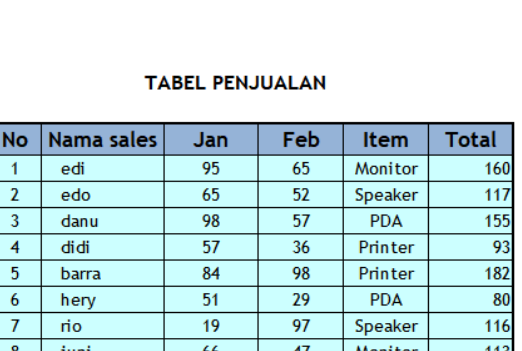
\includegraphics[width=57.12mm,height=96.53mm]{images/llm/page_026_img_02.png}%
\end{textblock*}

% deskripsi: Waveform audio berwarna biru
% bbox normalisasi: [0.0600, 0.5180, 0.9400, 0.9120]
\begin{textblock*}{184.80mm}(12.60mm,153.85mm)
\noindent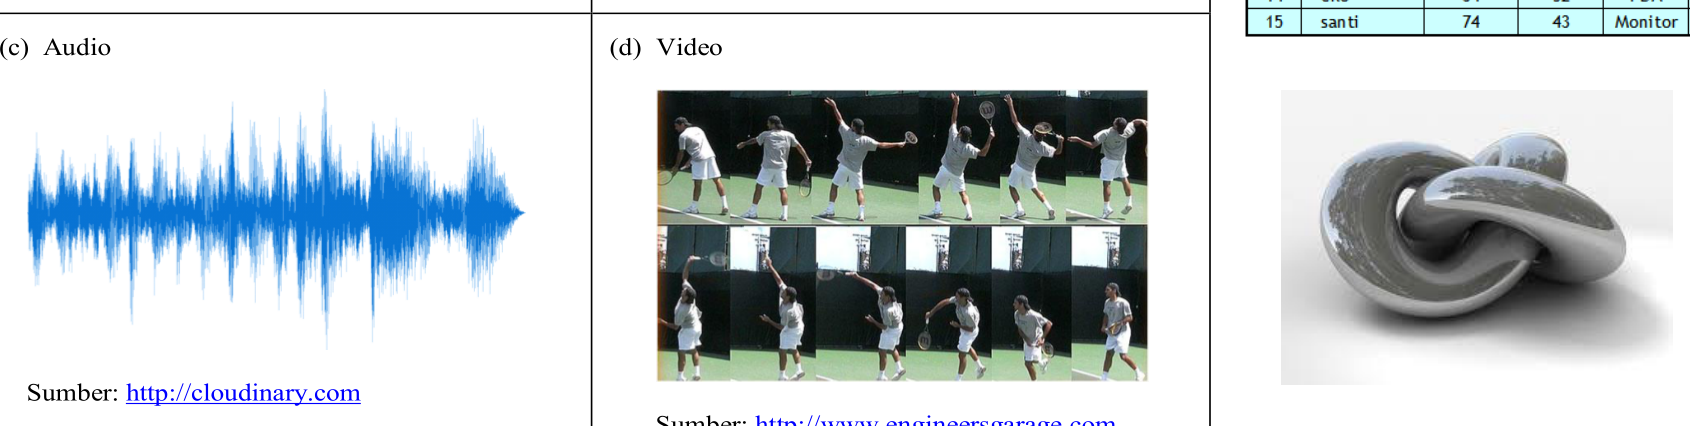
\includegraphics[width=184.80mm,height=117.02mm]{images/llm/page_026_img_03.png}%
\end{textblock*}

% deskripsi: Kumpulan frame video yang menunjukkan orang melakukan gerakan olahraga/senam
% bbox normalisasi: [0.4050, 0.5500, 0.6560, 0.8420]
\begin{textblock*}{52.71mm}(85.05mm,163.35mm)
\noindent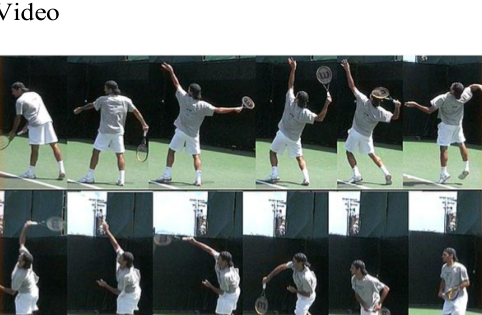
\includegraphics[width=52.71mm,height=86.72mm]{images/llm/page_026_img_04.png}%
\end{textblock*}

% deskripsi: Gambar rendering 3D berbentuk simpul logam mengkilap
% bbox normalisasi: [0.7360, 0.4200, 0.9130, 0.6850]
\begin{textblock*}{37.17mm}(154.56mm,124.74mm)
\noindent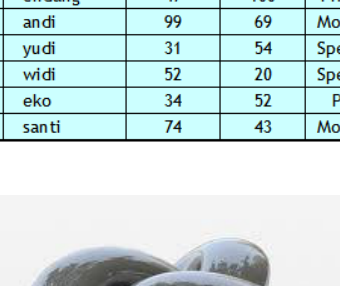
\includegraphics[width=37.17mm,height=78.71mm]{images/llm/page_026_img_05.png}%
\end{textblock*}

% bbox perkiraan otomatis: Foto berbagai macam paprika warna-warni
% bbox perkiraan otomatis: Waveform audio berwarna biru

\newpage

% --- unit llm 27 ---
% === Halaman 27 (llm) ===

\section*{2. Pengirim (sender) dan penerima (receiver)}

Pengirim: pihak yang mengirim pesan \\
Penerima (receiver): pihak yang menerima pesan

\begin{itemize}
    \item Di dalam kriptografi, pengirim pesan ditokohkan sebagai Alice dan penerima pesan ditokohkan sebagai Bob (agar terkesan lebih manusiawi ketimbang menggunakan simbol A, B, C, dan sebagainya).
\end{itemize}

\vspace{10mm}

% deskripsi: Ilustrasi komunikasi antara Alice sebagai pengirim dan Bob sebagai penerima dengan pertukaran pesan 'Halo'.
% bbox normalisasi: [0.2300, 0.6400, 0.7100, 0.8900]
\begin{textblock*}{100.80mm}(48.30mm,190.08mm)
\noindent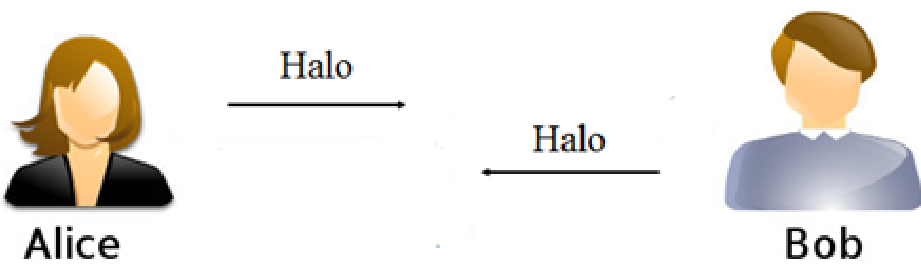
\includegraphics[width=100.80mm,height=74.25mm]{images/llm/page_027_img_01.png}%
\end{textblock*}

\newpage

% --- unit llm 28 ---
% === Halaman 28 (llm) ===

\section*{3. Penyusup (\textit{intruder})}
\begin{itemize}
    \item Pihak ketiga yang menyadap, mengintersepsi, menghapus, menambah, atau mengubah pesan
    \item Sebutan lain: \textit{eavesdropper, enemy, adversary, interceptor, bad guy}, dsb
    \item Nama tokohnya: Eve, Carol, Trudy, Mallory, dsb
\end{itemize}

\vspace{40mm}

Ronald Rivest: \textcolor{red}{"cryptography is about communication in the presence of adversaries"}

% deskripsi: Diagram ilustrasi komunikasi antara Alice dan Bob yang sedang dipantau oleh Eve sebagai eavesdropper.
% bbox normalisasi: [0.2300, 0.4700, 0.7300, 0.8800]
\begin{textblock*}{105.00mm}(48.30mm,139.59mm)
\noindent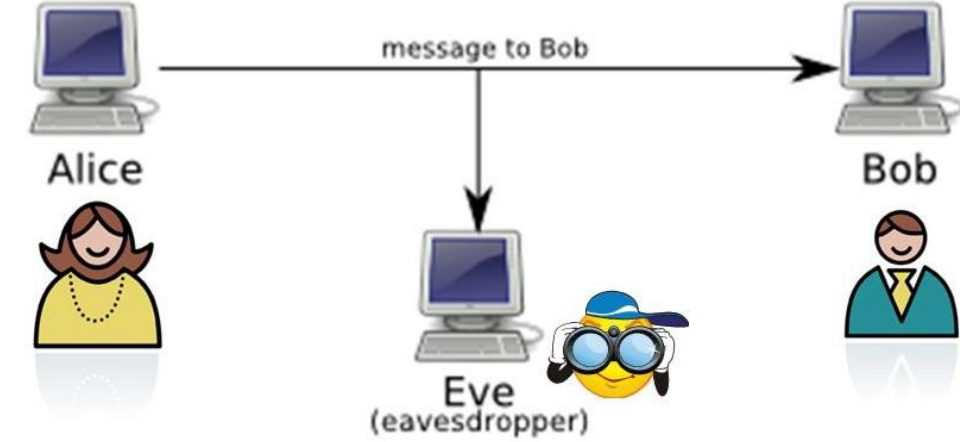
\includegraphics[width=105.00mm,height=121.77mm]{images/llm/page_028_img_01.png}%
\end{textblock*}

\newpage

% --- unit llm 29 ---
% === Halaman 29 (llm) ===

\textcolor{red}{Q:} What can a ``bad guy'' do?
\textcolor{red}{A:} a lot!
\begin{itemize}
    \item \textcolor{red}{eavesdrop}: intercept messages
    \item actively \textcolor{red}{insert} messages into connection
    \item \textcolor{red}{impersonation}: can fake (spoof) source address in packet (or any field in packet)
    \item \textcolor{red}{hijacking}: ``take over'' ongoing connection by removing sender or receiver, inserting himself in place
    \item \textcolor{red}{denial of service}: prevent service from being used by others (e.g., by overloading resources)
\end{itemize}

\vspace{10mm}
\hfill \textcolor{red}{Sumber: Chapter 8, Network Security}

\newpage

% --- unit llm 30 ---
% === Halaman 30 (llm) ===

4. \textbf{Cipherteks} (\textit{ciphertext}): pesan yang telah disandikan sehingga tidak bermakna lagi.

Tujuan: agar pesan tidak dapat dibaca oleh pihak yang tidak berhak.

Nama lain: \textbf{kriptogram} (\textit{cryptogram})

\begin{itemize}
    \item \textbf{Contoh:}
    \begin{itemize}
        \item \textbf{Plainteks:} \texttt{culik anak itu jam 11 siang}
        \item \textbf{Cipherteks:} \texttt{t\textasciicircum\$gfUi89rewoFpfdWqLMp[uTcxZ}
        \item \textbf{Kriptogram:} \texttt{t\textasciicircum\$gfU i89rewo FpfdWqLM p[uTcxZ}
    \end{itemize}
\end{itemize}

\newpage

% --- unit llm 31 ---
% === Halaman 31 (llm) ===

\textcolor{red}{Plainteks:}\vspace{2mm}
\begin{center}
\begin{tabular}{|p{0.6\textwidth}|}
\hline
Dinas Pendidikan Kota Ternate meminta kepada pihak sekolah dan orang tua siswa untuk jenjang pendidikan SD dan SMP se-Kota Ternate untuk melarang para siswa membawa permainan lato-lato yang sedang tren itu ke sekolah, karena akan mengganggu kegiatan belajar mengajar yang dinilai berbahaya sehingga mengantisipasi kecelakaan bagi anak di daerah itu.\hline
\end{tabular}
\end{center}
\vspace{10mm}
\textcolor{red}{Cipherteks:}\vspace{2mm}
\begin{center}
\begin{tabular}{|p{0.6\textwidth}|}
\hline
HAWFHZDOHAHANGOMKLGFCVWFLBOCPRKFGNHOFNIN \\ SPGNLHMPFVBEFWMVFWTBWRHSFZRWKFQMVHPAFWIK \\ DOHAHANGPFEWNFPNFKNLHMPFGLBAMGFCXKFQ MOCFV \\ AVKANIAVHSFZRNCODGAFOHYUVGWFOGFXEGFMLFWIT \\ HEFWTBVCPAYQOBLHMPFVBPVADOVWGNGFWOCKARVKA \\ RQOBRGGFFWCHFVGVYUDORVGVYCFWABAPVSVGCHGCI \\ DRFIFH BAPVQRVOCKAFWSGHSNIHSOBDHFVNGFWDGRGF \\ WGNHANFCVIDGSWZ \hline
\end{tabular}
\end{center}

\newpage

% --- unit llm 32 ---
% === Halaman 32 (llm) ===

\textcolor{red}{Plainteks}: \begin{center} \begin{tabular}{|p{0.7\textwidth}|} \hline Setelah Presiden Venezuela Nicolas Maduro digulingkan dan ditahan di New York atas tuduhan terorisme narkoba, kepemimpinan di Caracas kini berpindah tangan ke pemerintahan sementara yang dikawal Amerika Serikat (AS). Meski demikian, jaringan loyalis dan aparat keamanan yang menopang kekuasaan Maduro tetap aktif dan memiliki pengaruh besar. Bahkan, tercatat kini ada sepuluh orang yang memegang kendali negara kaya minyak itu, baik dari kubu Venezuela maupun AS. \\ \hline \end{tabular} \end{center} \vspace{10mm} \textcolor{red}{Cipherteks}: \begin{center} \begin{tabular}{|p{0.7\textwidth}|} \hline Ti2TVWlery8mUA6rmIz0IC17mXmlz1ykQH2D+rc5fgQyJkFyNfKcNbnOeJhS+s Ag3wyyPuiuR4xjdpvj0h7jQnzdjcLOj++ /jm6enh7KO6zOvg2RgVdgNcFyaUZZiZ/x+v /2ZmeYUrACii7TgdDb84ypbvSSwSZ32SuOn0JFurxB9ZUpSRHx8b17ff8bN6f/jgg0 E62YfwxExz+n+HzwS8jkSuPy8e42MRUnp8+OxVuZofItKhnT9ZTns+D2Sv/zFU9In wvLzu2oi+cyp8jHfyjWQvcKOSLkuFUTL5y4wM3F48J4Ht/RrGgaHOV7igXYCAT+FF ZlbjORyXpfl231fificW3K04Ssju1SG2Crnuwy6aqNx9WhYcUpaP925LFm5OY7Ne X Bcod0AmLd+GIOSf dzlBXwkpLJyFQNwN/SBWHow+RDW7xaZKOw1A2u1O7wPNB Dj6L73AlxmyhYzeY/+lg/4YFeSbxcoJK+kGYIOqYf0YITYHpKriPyLuA/DuA3OpvO BJCOOQjl2int4Q L0r7IpTk8vv10d+mgv5KcseGSnBJS pORngTWrNIaS6uFdOOYQKz NpWWduYUyZhirMM8dqmXGVimuRXWCuCGxUZ3SFO LglaJrke= \\ \hline \end{tabular} \end{center}

\newpage

% --- unit llm 33 ---
% === Halaman 33 (llm) ===

\vspace{215.03mm}

Plain-image \vspace{10mm} Cipher-image

% deskripsi: Gambar asli (plain-image) yang menampilkan beberapa kapal nelayan di pelabuhan dengan latar belakang mercusuar.
% bbox normalisasi: [0.0550, 0.1060, 0.4720, 0.8430]
\begin{textblock*}{87.57mm}(11.55mm,31.48mm)
\noindent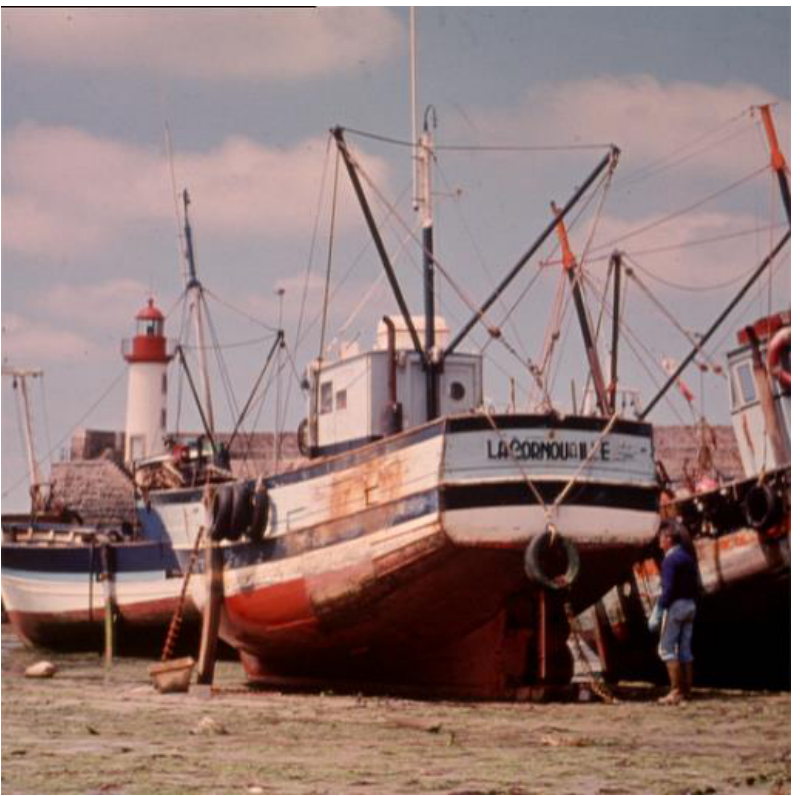
\includegraphics[width=87.57mm,height=218.89mm]{images/llm/page_033_img_01.png}%
\end{textblock*}

% deskripsi: Gambar terenkripsi (cipher-image) yang terlihat seperti noise acak berwarna-warni.
% bbox normalisasi: [0.5050, 0.1060, 0.9160, 0.8300]
\begin{textblock*}{86.31mm}(106.05mm,31.48mm)
\noindent
\includegraphics[width=86.31mm,height=215.03mm]{images/llm/page_033_img_02.png}%
\end{textblock*}

\newpage

% --- unit llm 34 ---
% === Halaman 34 (llm) ===

\vspace{154.44mm}

\vspace{60mm}
\begin{center}
Plain-video \hspace{6cm} Encrypted-video
\end{center}

% deskripsi: Gambar perbandingan antara video asli (Plain-video) yang menampilkan pria memakai helm proyek dan video yang telah terenkripsi (Encrypted-video) yang terlihat seperti noise berwarna.
% bbox normalisasi: [0.0970, 0.2100, 0.9160, 0.7300]
\begin{textblock*}{171.99mm}(20.37mm,62.37mm)
\noindent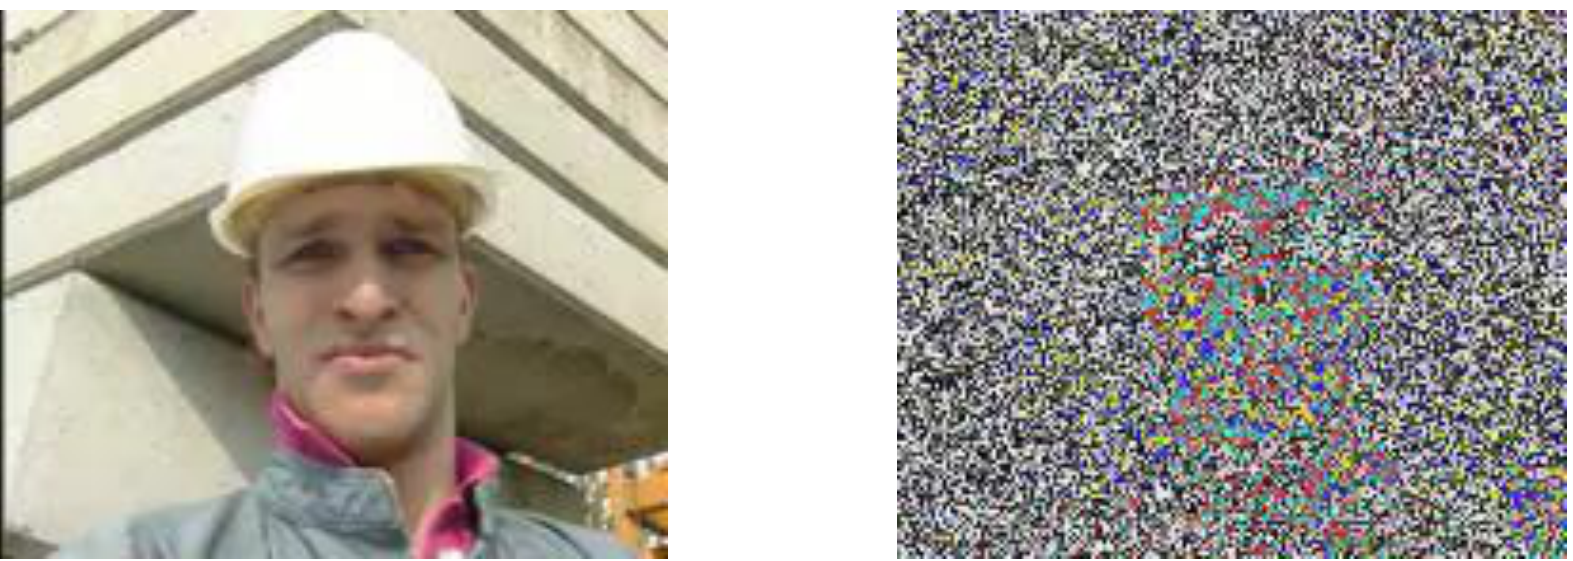
\includegraphics[width=171.99mm,height=154.44mm]{images/llm/page_034_img_01.png}%
\end{textblock*}

\newpage

% --- unit llm 35 ---
% === Halaman 35 (llm) ===

\textcolor{red}{Plainteks:}\vspace{2mm}
\begin{center}
\fbox{\parbox{0.6\textwidth}{Dinas Pendidikan Kota Ternate meminta kepada pihak sekolah dan orang tua siswa untuk jenjang pendidikan SD dan SMP se-Kota Ternate untuk melarang para siswa membawa permainan lato-lato yang sedang tren itu ke sekolah, karena akan mengganggu kegiatan belajar mengajar yang dinilai berbahaya sehingga mengantisipasi kecelakaan bagi anak di daerah itu.}}
\end{center}

\vspace{10mm}

\textcolor{red}{Cipherteks:}\vspace{2mm}
\begin{center}
\fbox{\parbox{0.6\textwidth}{HAWFHZDOHAHANGOMKLGF CVWFLBOCPRKFGNHOFNIN\\SPGNLHMPFVBEFWMVFWTBWRHSFZRWK FQMVHPAFWIK\\DOHAHANGPFEWNFPNFKNLHMPFGLBAMGFCXK FQ MOCFV\\AVKANIAVHSFZRN CODGAFOHYUVGWFOFGFXEG FMLFWIT\\HEFWTBVCPAYQOBLHMPFVBPVADOVWGN FWOCKARVKA\\RQOBRGGFFWCHFVGYUDORVGVYCFWABAPVSVGCHGCI\\DRFIFHBAPVQRVOCKAFWSGHSNIHSOBDHFVNGFWDGRGF\\WGNHANFCVIDGSWZ}}
\end{center}

% deskripsi: Kotak berisi teks plainteks dalam Bahasa Indonesia mengenai larangan permainan lato-lato di sekolah.
% bbox normalisasi: [0.2270, 0.3400, 0.8270, 0.4640]
\begin{textblock*}{126.00mm}(47.67mm,100.98mm)
\noindent
\includegraphics[width=126.00mm,height=36.83mm]{images/llm/page_035_img_01.png}%
\end{textblock*}

% deskripsi: Kotak berisi teks cipherteks yang terdiri dari rangkaian huruf kapital acak.
% bbox normalisasi: [0.2270, 0.5110, 0.8270, 0.9530]
\begin{textblock*}{126.00mm}(47.67mm,151.77mm)
\noindent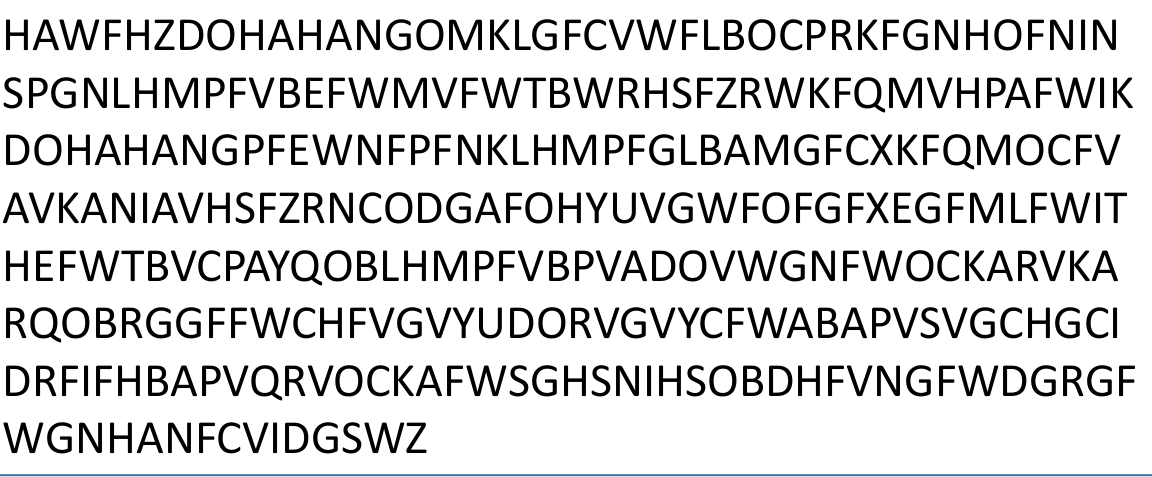
\includegraphics[width=126.00mm,height=131.27mm]{images/llm/page_035_img_02.png}%
\end{textblock*}

\newpage

% --- unit llm 36 ---
% === Halaman 36 (llm) ===

\textbf{5. Enkripsi (\textit{encryption}) dan dekripsi (\textit{decryption})}

\begin{itemize}
    \item Enkripsi: proses menyandikan plainteks menjadi cipherteks. \\ Nama lain: \textit{enciphering}
    \item Dekripsi: proses mengembalikan cipherteks menjadi plainteks semula. \\ Nama lain: \textit{deciphering}
\end{itemize}

\vspace{10mm}

% deskripsi: Diagram alur proses enkripsi dan dekripsi yang menunjukkan perubahan plainteks menjadi cipherteks melalui proses Enkripsi, kemudian kembali menjadi plainteks melalui proses Dekripsi.
% bbox normalisasi: [0.1540, 0.5560, 0.8080, 0.7140]
\begin{textblock*}{137.34mm}(32.34mm,165.13mm)
\noindent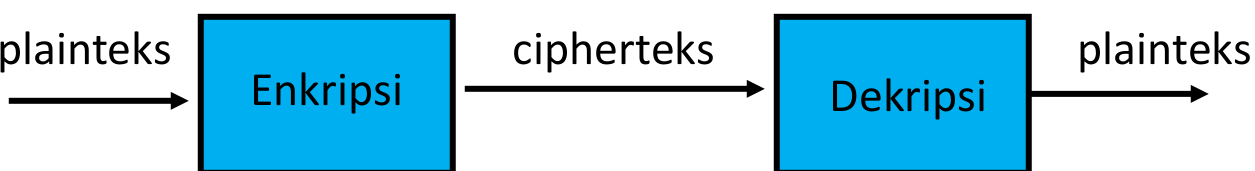
\includegraphics[width=137.34mm,height=46.93mm]{images/llm/page_036_img_01.png}%
\end{textblock*}

\newpage

% --- unit llm 37 ---
% === Halaman 37 (llm) ===

\vspace{163.35mm}

\begin{itemize}
  \item Meskipun Eve dapat menyadap komunikasi antara Alice dan Bob, namun karena pesan sudah dienkripsi menjadi cipherteks, Eve tidak dapat memahami pesan yang disadapnya
\end{itemize}
\vspace{10mm}

% deskripsi: Diagram proses enkripsi dan dekripsi pesan antara Alice dan Bob dengan Eve sebagai penyadap yang hanya melihat cipherteks.
% bbox normalisasi: [0.1900, 0.3600, 0.7400, 0.9100]
\begin{textblock*}{115.50mm}(39.90mm,106.92mm)
\noindent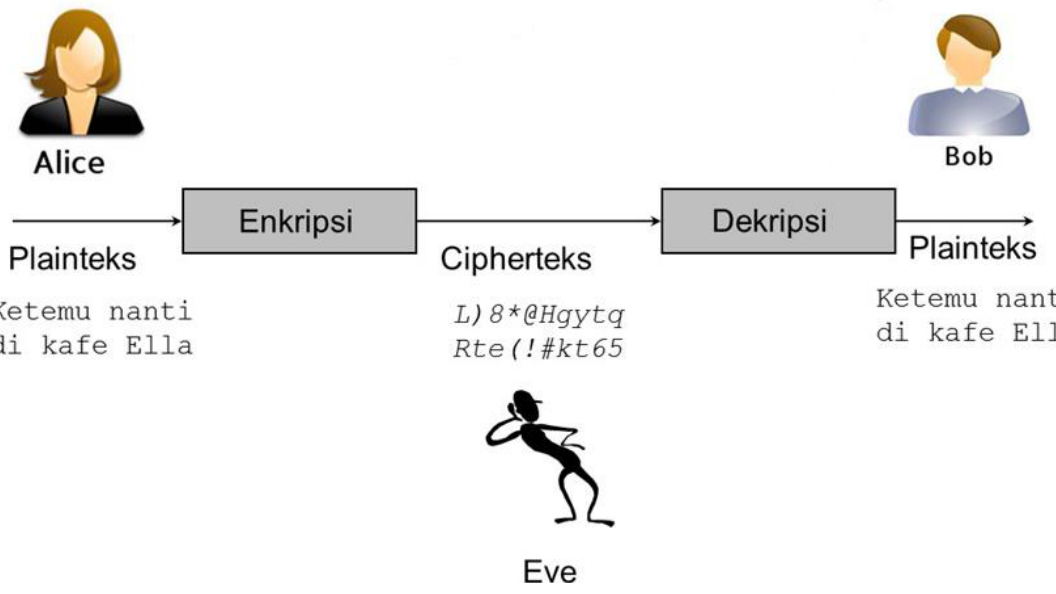
\includegraphics[width=115.50mm,height=163.35mm]{images/llm/page_037_img_01.png}%
\end{textblock*}

\newpage

% --- unit llm 38 ---
% === Halaman 38 (llm) ===

section{6. Kunci}

\begin{itemize}
    \item Agar enkripsi dan dekripsi hanya dapat dilakukan oleh dua pihak yang berkomunikasi, maka diperlukan \textbf{kunci} rahasia.
    \item Kunci adalah parameter yang digunakan di dalam enkripsi dan dekripsi\\
    Simbol: K ( K dapat berupa integer, string, alphanumeric, dsb )
\end{itemize}

\vspace{83.16mm}

\[ \text{Enkripsi: } E_K(P) = C \quad ; \quad \text{Dekripsi: } D_K(C) = P \]

\vspace{30mm}

\textbf{Prinsip Kherkoff}: semua algoritma kriptografi harus publik (tidak rahasia), hanya kunci yang harus rahasia.

% deskripsi: Diagram alir proses enkripsi dan dekripsi yang menunjukkan aliran dari Plainteks melalui proses Enkripsi (menggunakan Kunci) menjadi Cipherteks, lalu melalui proses Dekripsi (menggunakan Kunci) kembali menjadi Plainteks.
% bbox normalisasi: [0.1440, 0.4600, 0.8200, 0.7400]
\begin{textblock*}{141.96mm}(30.24mm,136.62mm)
\noindent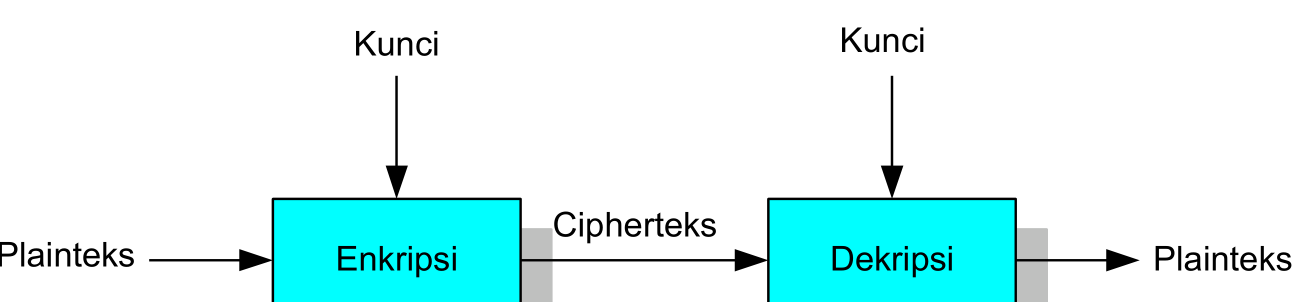
\includegraphics[width=141.96mm,height=83.16mm]{images/llm/page_038_img_01.png}%
\end{textblock*}

\newpage

% --- unit llm 39 ---
% === Halaman 39 (llm) ===

% (tidak ada teks dari model)

% deskripsi: Diagram proses enkripsi dan dekripsi simetris yang menunjukkan aliran pesan dari plainteks 'Kirim senjata perang P', melalui proses Enkripsi $E_K(P) = C$ dengan kunci 'ocean' menjadi cipherteks 'Stype xouvatx kutreq C', lalu proses Dekripsi $D_K(C) = P$ dengan kunci yang sama kembali menjadi plainteks 'Kirim senjata perang P'.
% bbox normalisasi: [0.0700, 0.3020, 0.9320, 0.6530]
\begin{textblock*}{181.02mm}(14.70mm,89.69mm)
\noindent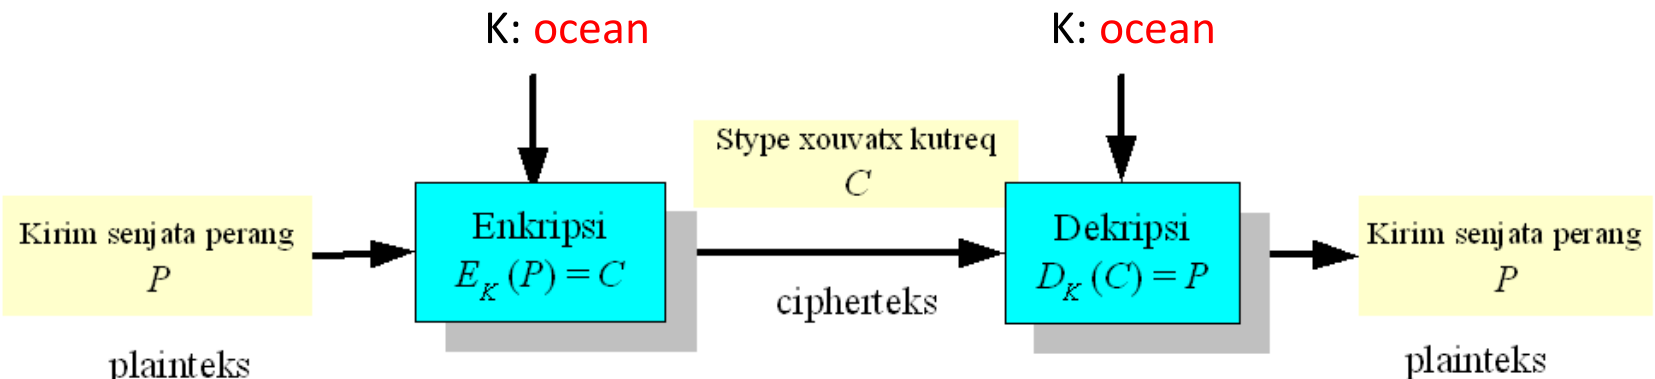
\includegraphics[width=181.02mm,height=104.25mm]{images/llm/page_039_img_01.png}%
\end{textblock*}

\newpage

% --- unit llm 40 ---
% === Halaman 40 (llm) ===

\section*{7. Cipher}

\begin{itemize}
    \item Algoritma untuk enkripsi dan dekripsi pesan
    \item Aturan (\textit{rule}) untuk \textit{enchipering} dan \textit{dechipering}, atau berupa fungsi matematika yang digunakan untuk enkripsi dan dekripsi pesan.
\end{itemize}

Contoh:
\begin{itemize}
    \item Enkripsi: Geser tiga huruf ke kanan \quad (rule)
    \item Dekripsi: Geser tiga huruf ke kiri \quad (rule)
    \item \[ E(p) = (p + k) \pmod{26} \quad(\text{fungsi matematika}) \]
    \item \[ D(c) = (c - k) \pmod{26} \quad(\text{fungsi matematika}) \]
\end{itemize}

\begin{itemize}
    \item \textcolor{red}{Classical cipher}: Caesar cipher, Vigenere cipher, Playfair Cipher, Enigma cipher, dll
    \item \textcolor{red}{Modern cipher}: DES, AES, Blowfish, Serpent, RSA, ElGamal, RC4, RC5, A5, dll
\end{itemize}

\newpage

% --- unit llm 41 ---
% === Halaman 41 (llm) ===

\section*{8. Sistem kriptografi (cryptosystem)}

Sistem kriptografi adalah $quintuple$ $(\mathcal{E}, \mathcal{D}, \mathcal{M}, \mathcal{K}, \mathcal{C})$
\begin{itemize}
    \item $\mathcal{M}$ adalah himpunan plainteks
    \item $\mathcal{K}$ adalah himpunan kunci
    \item $\mathcal{C}$ adalah himpunan cipherteks
    \item $\mathcal{E}$ adalah himpunan fungsi enkripsi $E: \mathcal{M} \times \mathcal{K} \to \mathcal{C}$
    \item $\mathcal{D}$ adalah himpunan fungsi dekripsi $D: \mathcal{C} \times \mathcal{K} \to \mathcal{M}$
\end{itemize}

\newpage

% --- unit llm 42 ---
% === Halaman 42 (llm) ===

Contoh: Caesar cipher (ingat kembali materi di dalam kuliah Matdis $\smiley$ )
\begin{itemize}
    \item $\mathcal{M} = \{ \text{huruf-huruf alfabet} \}$
    \item $\mathcal{K} = \{ k \mid k \text{ adalah bilangan bulat dan } 0 \le k \le 25 \}$
    \item $\mathcal{E} = \{ E_k \mid k \in \mathcal{K} \text{ dan untuk semua plainteks } m, \\
    [ E_k(m) = (m + k) \pmod{26} ]$
    \item $\mathcal{D} = \{ D_k \mid k \in \mathcal{K} \text{ dan untuk semua cipherteks } c, \\
    [ D_k(c) = (c - k) \pmod{26} ]$
    \item $\mathcal{C} = \mathcal{M}$
\end{itemize}

\newpage

% --- unit llm 43 ---
% === Halaman 43 (llm) ===

\begin{center}
\Huge Dua Aplikasi Utama Enkripsi
\end{center}

\begin{itemize}
    \item Enkripsi dokumen di dalam storage (\textit{encryption at rest})
    \item Enkripsi pesan yang dikirim (\textit{encryption on motion})
\end{itemize}

\vspace{70mm}

Sumber: \url{https://www.scienceabc.com/innovation/how-whatsapp-app-message-end-to-end-encryption-works-msgs-security-method-key.html}

% deskripsi: Screenshot jendela dialog 'Encrypt Document' yang menampilkan kolom input password dan peringatan tentang kehilangan password.
% bbox normalisasi: [0.0500, 0.4400, 0.4600, 0.8800]
\begin{textblock*}{86.10mm}(10.50mm,130.68mm)
\noindent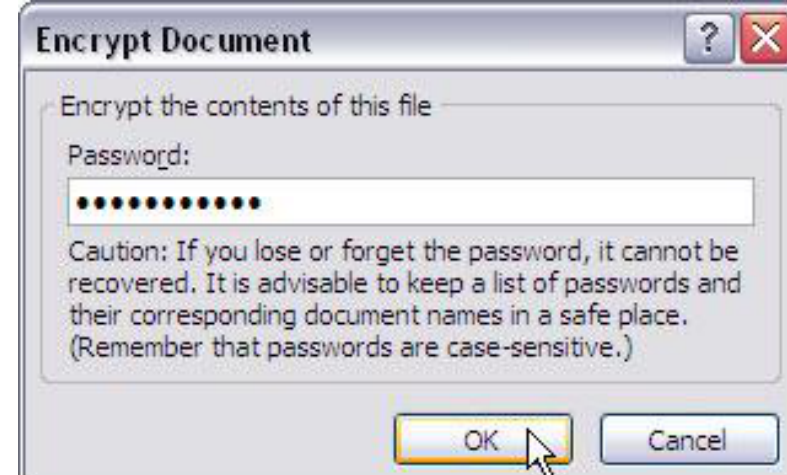
\includegraphics[width=86.10mm,height=130.68mm]{images/llm/page_043_img_01.png}%
\end{textblock*}

% deskripsi: Foto layar smartphone yang menampilkan percakapan WhatsApp dengan notifikasi bahwa pesan diamankan dengan enkripsi end-to-end.
% bbox normalisasi: [0.5300, 0.4300, 0.9100, 0.8800]
\begin{textblock*}{79.80mm}(111.30mm,127.71mm)
\noindent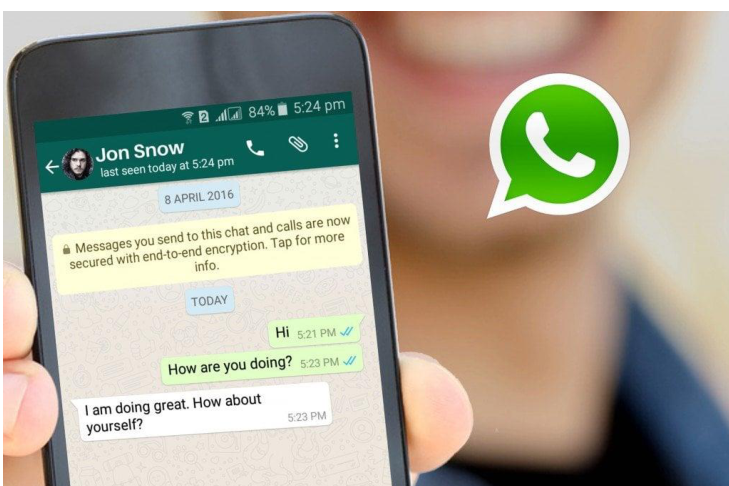
\includegraphics[width=79.80mm,height=133.65mm]{images/llm/page_043_img_02.png}%
\end{textblock*}

\newpage

% --- unit llm 44 ---
% === Halaman 44 (llm) ===

\section*{Kriptanalisis}

\begin{itemize}
    \item \textbf{Kriptanalisis} (\textit{cryptanalysis}): ilmu dan seni untuk memecahkan chiperteks menjadi plainteks tanpa mengetahui \textit{kunci} yang digunakan.
    \item Pelakunya disebut \textbf{kriptanalis}
    \item Kriptanalisis merupakan "lawan" kriptografi
    \item Teknik kriptanalisis sudah ada sejak abad ke-9.
\end{itemize}

\vspace{10mm}

Kriptanalisis dikemukakan pertama kali oleh seorang ilmuwan Arab pada Abad IX bernama \textit{Abu Yusuf Yaqub Ibnu Ishaq Ibnu As-Sabbah Ibnu 'Omran Ibnu Ismail Al-Kindi}, atau yang lebih dikenal sebagai \textbf{Al-Kindi}.

% deskripsi: Gambar prangko yang menampilkan ilustrasi Al-Kindi sedang menulis
% bbox normalisasi: [0.6780, 0.3980, 0.8670, 0.8630]
\begin{textblock*}{39.69mm}(142.38mm,118.21mm)
\noindent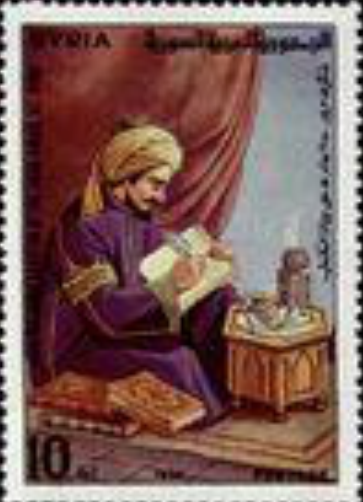
\includegraphics[width=39.69mm,height=138.10mm]{images/llm/page_044_img_01.png}%
\end{textblock*}

\newpage

% --- unit llm 45 ---
% === Halaman 45 (llm) ===

\vspace{207.31mm}

\begin{itemize}
    \item Al-Kindi menulis buku tentang seni memecahkan kode, buku yang berjudul 'Risalah fi Istikhraj al-Mu'amma (Manuscript for the Deciphering Cryptographic Messages)
    \item Al-Kindi menemukan frekuensi perulangan huruf di dalam Al-Quran. Teknik yang digunakan Al-Kindi kelak dinamakan \textbf{analisis frekuensi}.
    \item Yaitu teknik untuk memecahkan cipherteks berdasarkan frekuensi kemunculan karakter di dalam pesan
\end{itemize}

\vspace{20mm}

\textcolor{red}{Halaman pertama buku Al-Kindi, Manuscript for the Deciphering Cryptographic}

% deskripsi: Screenshot halaman pertama manuskrip bahasa Arab karya Al-Kindi tentang dekripsi pesan kriptografis.
% bbox normalisasi: [0.6160, 0.0670, 0.8030, 0.7650]
\begin{textblock*}{39.27mm}(129.36mm,19.90mm)
\noindent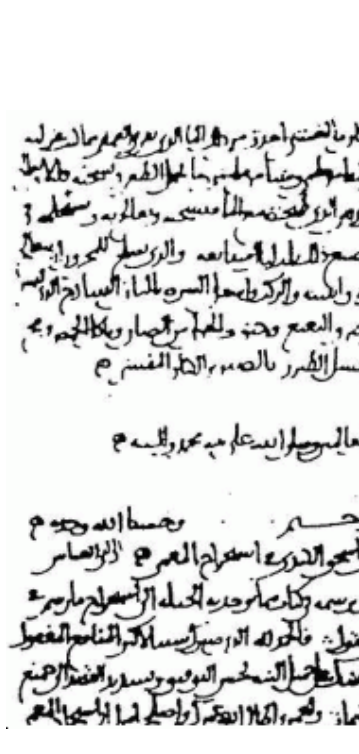
\includegraphics[width=39.27mm,height=207.31mm]{images/llm/page_045_img_01.png}%
\end{textblock*}

\newpage

% --- unit llm 46 ---
% === Halaman 46 (llm) ===

\vspace{238.79mm}

Sejarah kriptanalisis mencatat hasil gemilang seperti pemecahan Telegram Zimmermann yang membawa Amerika Serikat ke kancah Perang Dunia I.\vspace{20mm}
\textcolor{red}{Telegram Zimmerman yang sudah berhasil didekripsi (Sumber: Wikipedia.org)}

% deskripsi: Screenshot dokumen Telegram Zimmermann yang telah didekripsi dalam bahasa Inggris.
% bbox normalisasi: [0.0600, 0.1080, 0.9400, 0.9120]
\begin{textblock*}{184.80mm}(12.60mm,32.08mm)
\noindent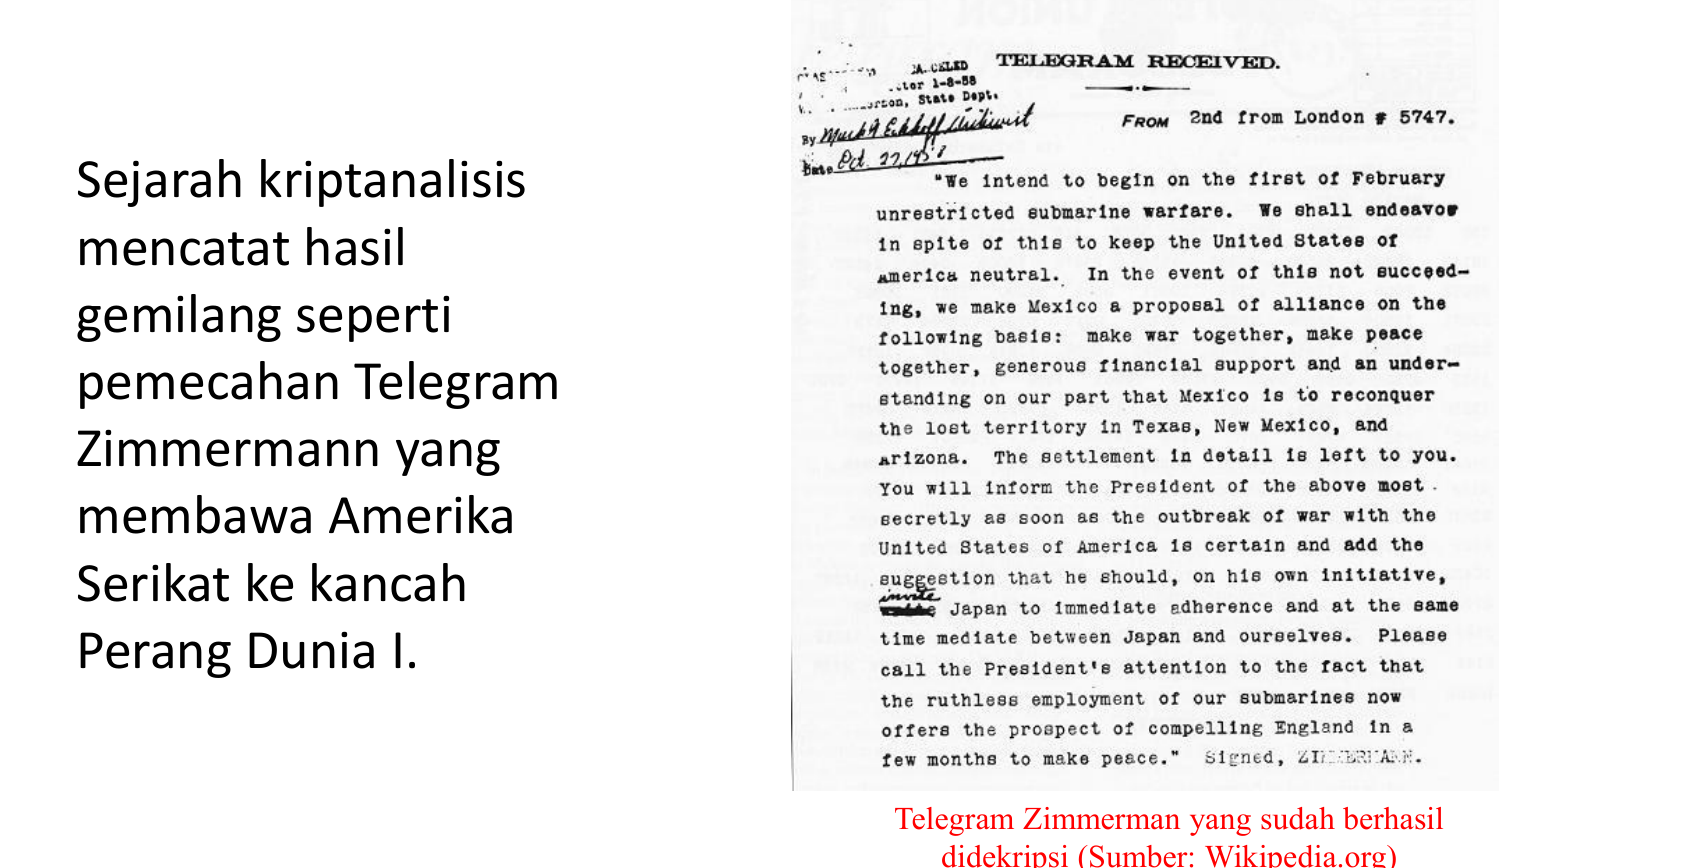
\includegraphics[width=184.80mm,height=238.79mm]{images/llm/page_046_img_01.png}%
\end{textblock*}

% bbox perkiraan otomatis: Screenshot dokumen Telegram Zimmermann yang telah didekripsi dalam bahasa Inggris.

\newpage

% --- unit llm 47 ---
% === Halaman 47 (llm) ===

\section*{Kriptologi}

\vspace{166.91mm}

Kriptologi (\textit{cryptology}): studi mengenai kriptografi dan kriptanalisis.

\vspace{50mm}

% deskripsi: Diagram hierarki yang menunjukkan Kriptologi terbagi menjadi dua cabang utama: Kriptografi (ilmu dan seni untuk menjaga keamanan pesan) dan Kriptanalisis (ilmu dan seni untuk memecahkan cipherteks), dengan panah dua arah yang menghubungkan keduanya.
% bbox normalisasi: [0.1870, 0.3680, 0.7860, 0.9300]
\begin{textblock*}{125.79mm}(39.27mm,109.30mm)
\noindent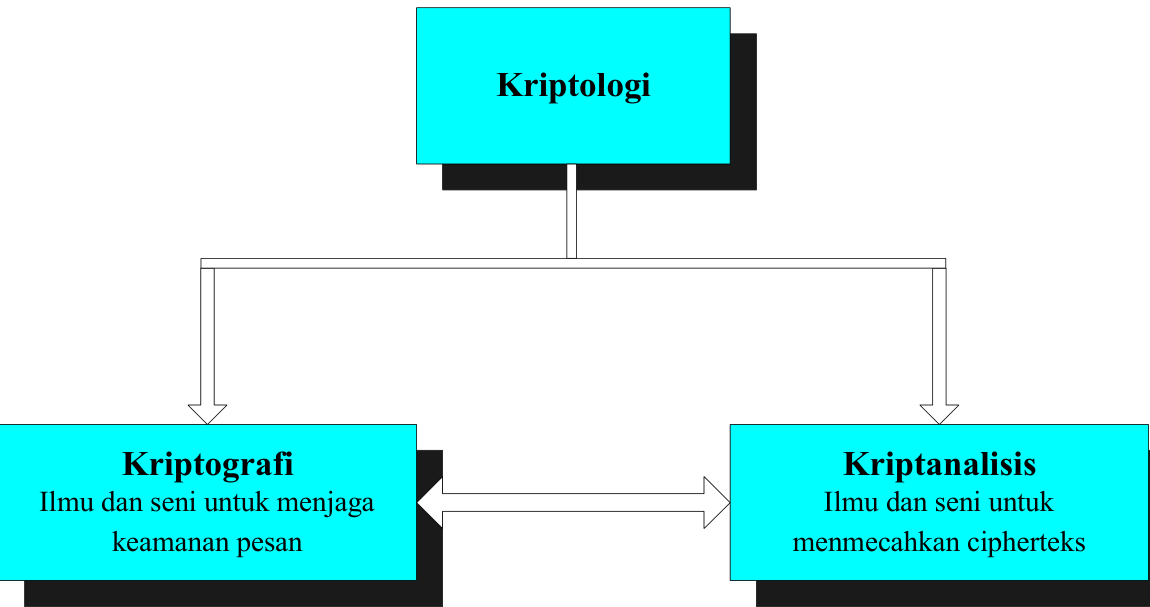
\includegraphics[width=125.79mm,height=166.91mm]{images/llm/page_047_img_01.png}%
\end{textblock*}

\newpage

% --- unit llm 48 ---
% === Halaman 48 (llm) ===

\section*{Sejarah Kriptografi}

\begin{itemize}
    \item Kriptografi sudah berusia sangat tua, sudah ada sejak peradaban manusia di bumi
    \item Secara historis, kriptografi diasosiasikan dengan kegiatan mata-mata, pemerintahan, dan militer, dan telah digunakan di dalam perang selama ribuan tahun.
    \item Tiga pihak yang memiliki kontribusi penting di dalam perkembangan kriptografi zaman dahulu: kalangan militer, diplomat, dan \textit{diarist}.
    \item Sejak lebih dari 50 tahun yang lalu, kriptografi mendapatkan landasan matematika, dan telah bergeser dari aplikasi militer ke aplikasi komersil.
    \item Secara garis besar, kriptografi dibagi menjadi dua era: \textcolor{red}{kriptografi klasik} dan \textcolor{red}{kriptografi modern}.
\end{itemize}

\newpage

% --- unit llm 49 ---
% === Halaman 49 (llm) ===

\vspace{238.79mm}

\section*{Old Cryptography}

\begin{itemize}
    \item \textit{Ancient cryptography} atau \textit{classical cryptography}
    \item Kriptografi zaman dulu (sebelum Masehi s/d sebelum ada komputer digital)
    \item Hanya mengenkripsi huruf dan angka, menggunakan kertas dan pena saja
    \item Semua \textit{cipher} nya sudah kadaluarsa (sudah tidak aman, karena sudah berhasil dikriptanalisis)
\end{itemize}

\vspace{10mm}

\begin{itemize}
    \item Caesar cipher
    \item Vigenere cipher
    \item Playfair cipher
    \item Hill cipher
    \item Beauford cipher
    \item Enigma cipher
    \item dll
\end{itemize}

% deskripsi: Ilustrasi gulungan papirus kuno dengan huruf-huruf di atasnya yang merepresentasikan kriptografi kuno.
% bbox normalisasi: [0.6900, 0.0000, 0.9950, 0.2430]
\begin{textblock*}{64.05mm}(144.90mm,0.00mm)
\noindent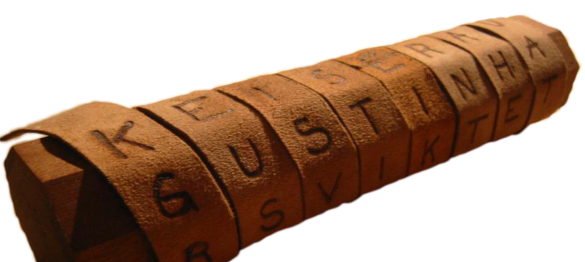
\includegraphics[width=64.05mm,height=72.17mm]{images/llm/page_049_img_01.png}%
\end{textblock*}

% deskripsi: Foto alat enkripsi cakram alfabet (cipher disk) yang digunakan untuk metode Caesar cipher.
% bbox normalisasi: [0.0600, 0.1080, 0.9400, 0.9120]
\begin{textblock*}{184.80mm}(12.60mm,32.08mm)
\noindent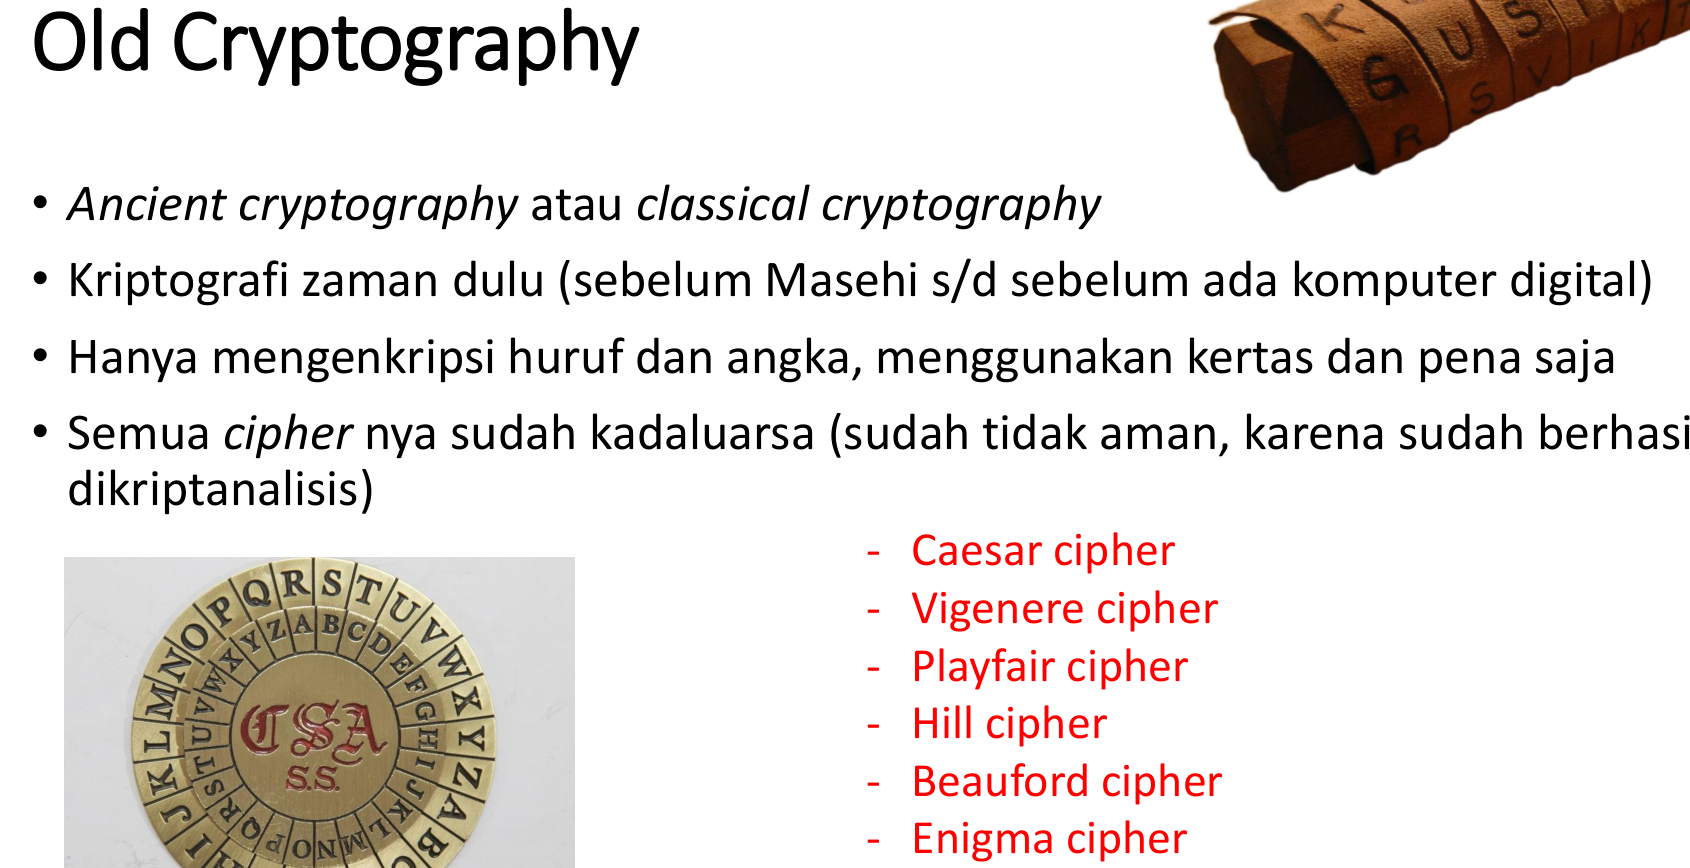
\includegraphics[width=184.80mm,height=238.79mm]{images/llm/page_049_img_02.png}%
\end{textblock*}

% bbox perkiraan otomatis: Foto alat enkripsi cakram alfabet (cipher disk) yang digunakan untuk metode Caesar cipher.

\newpage

% --- unit llm 50 ---
% === Halaman 50 (llm) ===

\section*{Modern Cryptography}
\begin{itemize}
    \item Enkripsi dan dekripsi pesan dalam bentuk digital dengan komputer digital
\end{itemize}

\noindent 1. Teks \vspace{40mm}

\vspace{99.79mm}

\noindent 2. Audio \vspace{10mm}

\noindent 3. Gambar (\textit{image})
\begin{itemize}
    \item DES, 3DES
    \item AES, Serpent
    \item RSA, ElGamal, ECC
    \item Diffie-Hellman
    \item MD5, SHA-3
    \item DSA
    \item TLS
    \item dll
\end{itemize}

\vspace{69.50mm}

\noindent 4. Video

% deskripsi: Contoh teks yang digunakan sebagai data untuk enkripsi: 'A Quick Brown Fox Jumps Over The Lazy Dog 0123456789'
% bbox normalisasi: [0.0670, 0.2880, 0.4860, 0.6250]
\begin{textblock*}{87.99mm}(14.07mm,85.54mm)
\noindent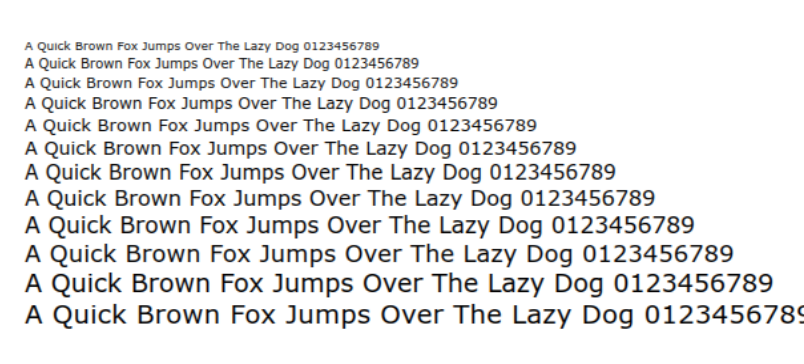
\includegraphics[width=87.99mm,height=100.09mm]{images/llm/page_050_img_01.png}%
\end{textblock*}

% deskripsi: Grafik bentuk gelombang audio (waveform) sebagai contoh data digital
% bbox normalisasi: [0.0540, 0.7040, 0.4330, 0.9350]
\begin{textblock*}{79.59mm}(11.34mm,209.09mm)
\noindent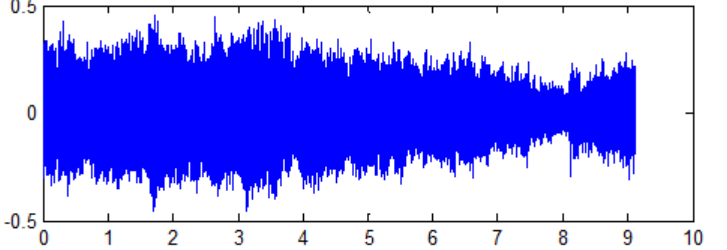
\includegraphics[width=79.59mm,height=68.61mm]{images/llm/page_050_img_02.png}%
\end{textblock*}

% deskripsi: Foto Taj Mahal sebagai contoh data gambar (image) yang akan dienkripsi
% bbox normalisasi: [0.5180, 0.2890, 0.6890, 0.6250]
\begin{textblock*}{35.91mm}(108.78mm,85.83mm)
\noindent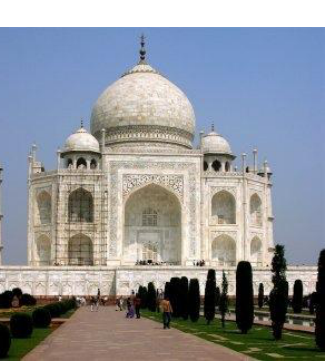
\includegraphics[width=35.91mm,height=99.79mm]{images/llm/page_050_img_03.png}%
\end{textblock*}

% deskripsi: Cuplikan frame video yang menunjukkan dua orang sebagai contoh data video
% bbox normalisasi: [0.5170, 0.7380, 0.8550, 0.9720]
\begin{textblock*}{70.98mm}(108.57mm,219.19mm)
\noindent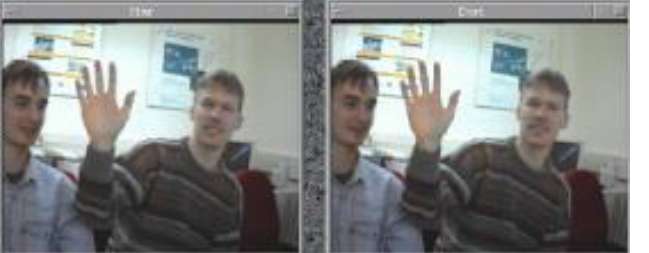
\includegraphics[width=70.98mm,height=69.50mm]{images/llm/page_050_img_04.png}%
\end{textblock*}

\newpage

% --- unit llm 51 ---
% === Halaman 51 (llm) ===

\section*{Kriptografi pada zaman Mesir Kuno}

\vspace{163.05mm}

\begin{itemize}
    \item Bangsa Mesir 4000 tahun yang lalu menggunakan \textit{hieroglyph} yang tidak standard untuk menulis pesan di dinding piramid.
\end{itemize}

\vspace{5mm}

% deskripsi: Foto prasasti dengan tulisan hieroglif Mesir Kuno yang dipahat pada permukaan batu.
% bbox normalisasi: [0.2330, 0.3930, 0.7310, 0.9420]
\begin{textblock*}{104.58mm}(48.93mm,116.72mm)
\noindent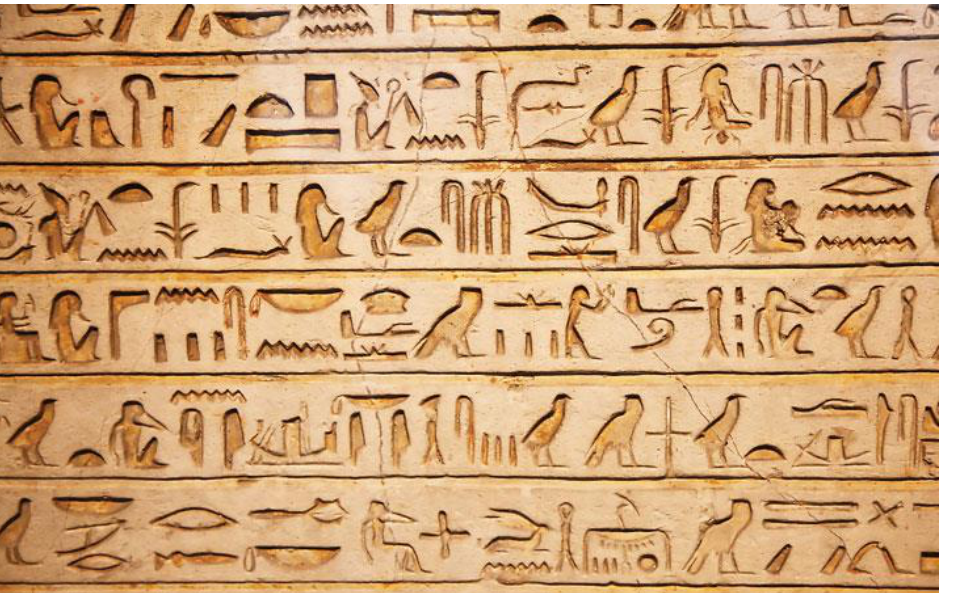
\includegraphics[width=104.58mm,height=163.05mm]{images/llm/page_051_img_01.png}%
\end{textblock*}

\newpage

% --- unit llm 52 ---
% === Halaman 52 (llm) ===

\section*{Kriptografi pada Zaman Yunani dan Romawi Kuno}

\begin{itemize}
    \item Di Yunani, kriptografi sudah digunakan 400 BC
    \item Alat yang digunakan: scytale
\end{itemize}

\vspace{40mm}

Plainteks: KILLKINGTOMORROWMIDNIGHT \\
Ciphrteks: KIMWIINOMGLGRIHLTRDTKOON

% deskripsi: Ilustrasi scytale yang memperlihatkan pita kertas tergulung dengan teks terenkripsi 'KILL KING TOMORROW MIDNIGHT'.
% bbox normalisasi: [0.1800, 0.4900, 0.4800, 0.7400]
\begin{textblock*}{63.00mm}(37.80mm,145.53mm)
\noindent
\includegraphics[width=63.00mm,height=74.25mm]{images/llm/page_052_img_01.png}%
\end{textblock*}

% deskripsi: Ilustrasi dua prajurit Yunani kuno sedang menggunakan alat scytale untuk berkomunikasi secara rahasia.
% bbox normalisasi: [0.5400, 0.4200, 0.8400, 0.7800]
\begin{textblock*}{63.00mm}(113.40mm,124.74mm)
\noindent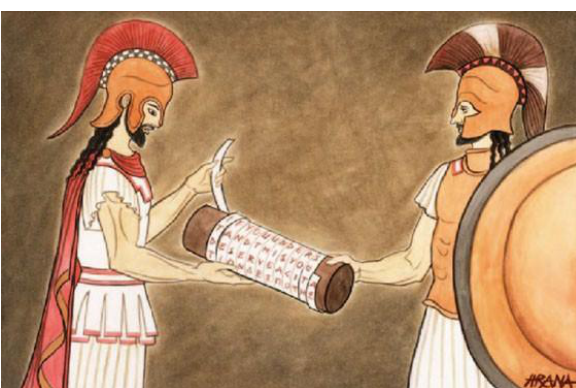
\includegraphics[width=63.00mm,height=106.92mm]{images/llm/page_052_img_02.png}%
\end{textblock*}

\newpage

% --- unit llm 53 ---
% === Halaman 53 (llm) ===

\vspace{250.07mm}

\section*{Kriptografi pada Bangsa Arab}

Sejarah kriptologi pada bangsa Arab dapat dibaca pada seri buku \textit{Arabic Origins of Cryptology} yang diterbitkan oleh \textit{King Faisal Center for Research and Islamic Studies}, Arab Saudi.

\vspace{40mm}

Ibn ad-Durayhim bernama lengkap Ali ibn Muhammad ibn Abd al Aziz, Tag ad-Din. Dia lahir di Mosul, Irak, pada bulan Sya'ban tahun 712 H atau 1312 M. Dia sering berdagang antara Kairo dan Damaskus dan ditunjuk sebagai guru di Masjid Umayah Damaskus. Dia pindah ke Mesir tahun 760 H/1359 M dan dikirim oleh Sultan sebagai duta kepada raja Abyssinia (sekarang Etiopia).

% deskripsi: Sampul buku berjudul 'Arabic Origins of Cryptology Volume Three: ibn ad-Durayhim's Treatise on Cryptanalysis'
% bbox normalisasi: [0.6120, 0.0340, 0.9570, 0.8760]
\begin{textblock*}{72.45mm}(128.52mm,10.10mm)
\noindent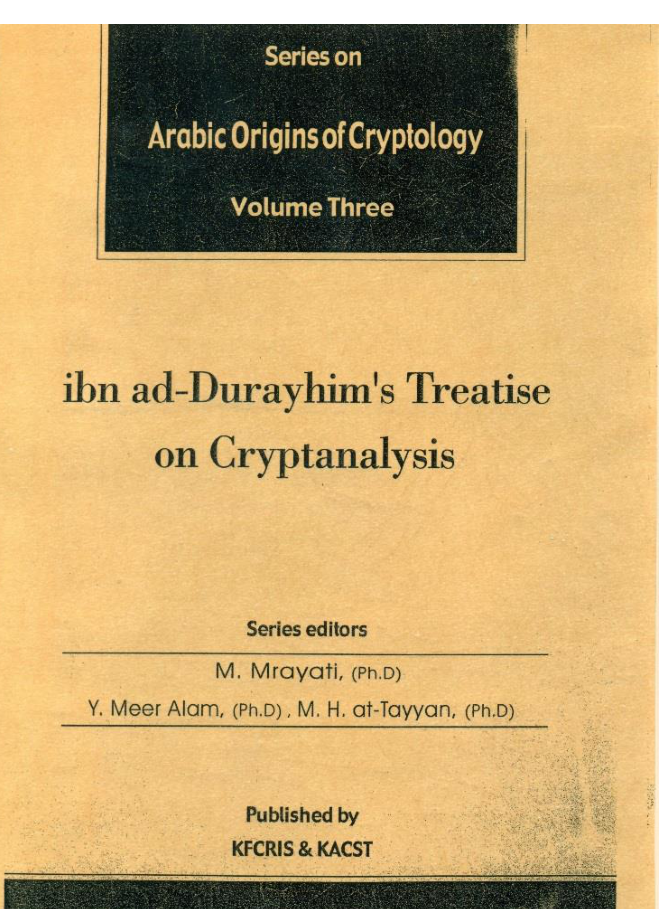
\includegraphics[width=72.45mm,height=250.07mm]{images/llm/page_053_img_01.png}%
\end{textblock*}

\newpage

% --- unit llm 54 ---
% === Halaman 54 (llm) ===

Menurut ad-Durayhim, jenis-jenis \textit{cipher} dapat dikelompokkan ke dalam delapan tipe:
\begin{enumerate}
  \item transposisi,
  \item substitusi,
  \item penambahan atau reduksi jumlah huruf,
  \item penggunaan piranti sandi,
  \item penggantian huruf dengan angka yang diboboti secara desimal,
  \item penyandian huruf dengan menggunakan kata-kata,
  \item penggantian huruf dengan nama generik,
  \item menggunakan simbol atau tanda untuk menyatakan huruf.
\end{enumerate}

\vspace{10mm}

\textcolor{red}{\textit{Cryptology was born among Arabs. They were the first to discover and write down the methods of cryptanalysis.}}
\textcolor{red}{(David Kahn -- Penulis buku: The Code Breaker)}

\newpage

% --- unit llm 55 ---
% === Halaman 55 (llm) ===

\textbf{Kriptografi di Eropa dari Zaman Renaisans sampai Abad 19}

\begin{itemize}
    \item Zaman renaisans $\rightarrow$ abad pertengahan (abad 15-16)
    \item \textit{Cipher} terkenal pada abad pertengahan hingga abad 19:
    \begin{enumerate}
        \item \textit{Vigenere Cipher}\
        Dipublikasikan oleh diplomat Perancis bernama Blaise de Vigenere pada tahun 1586.
        \vspace{5mm}
        \item \textit{Playfair Cipher}\
        Dipromosikan oleh diplomat Inggris, Lord Playfair, meskipun penemu aslinya adalah Charles Wheatstone pada tahun 1854.
    \end{enumerate}
\end{itemize}

\newpage

% --- unit llm 56 ---
% === Halaman 56 (llm) ===

\vspace{160.68mm}

\begin{itemize}
  \item Pada Abad ke-17, sejarah kriptografi pernah mencatat korban di Inggris.
  \item Queen Mary of Scotland, dipancung setelah pesan rahasianya dari balik penjara (sebuah cipherteks yang isinya rencana membunuh Ratu Elizabeth I) pada Abad Pertengahan berhasil dipecahkan oleh Thomas Phelippes, seorang pemecah kode (codebreaker).
\end{itemize}

% deskripsi: Potret Queen Mary of Scotland
% bbox normalisasi: [0.6660, 0.2020, 0.9120, 0.7430]
\begin{textblock*}{51.66mm}(139.86mm,59.99mm)
\noindent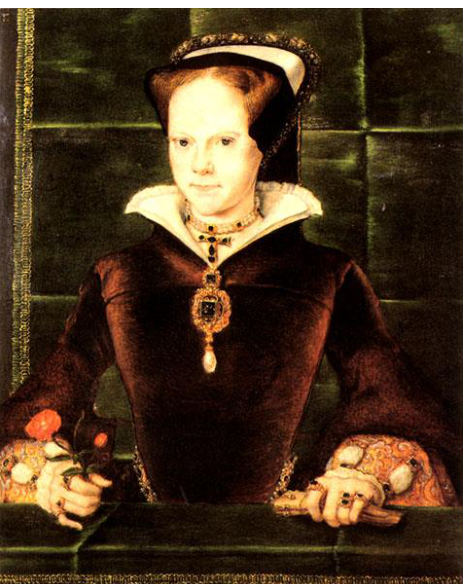
\includegraphics[width=51.66mm,height=160.68mm]{images/llm/page_056_img_01.png}%
\end{textblock*}

\newpage

% --- unit llm 57 ---
% === Halaman 57 (llm) ===

\vspace{237.01mm}

\section*{Kriptografi pada Perang Dunia II}

\begin{itemize}
    \item Perang Dunia ke II, Pemerintah Nazi Jerman membuat mesin enkripsi yang dinamakan \textit{Enigma}.
    \item \textit{Enigma cipher} berhasil dipecahkan oleh pihak Sekutu.
    \item Keberhasilan memecahkan \textit{Enigma} sering dikatakan sebagai faktor yang memperpendek perang dunia ke-2
\end{itemize}

\vspace{20mm}

\begin{center}
    Enigma
\end{center}

% deskripsi: Foto mesin Enigma dengan berbagai label keterangan bagian-bagian mesin seperti spare light bulbs, viewing windows, rotor cylinder, position of rotors, plugboard, keyboard, dan alphabetical lightboard.
% bbox normalisasi: [0.5370, 0.0740, 0.9660, 0.8720]
\begin{textblock*}{90.09mm}(112.77mm,21.98mm)
\noindent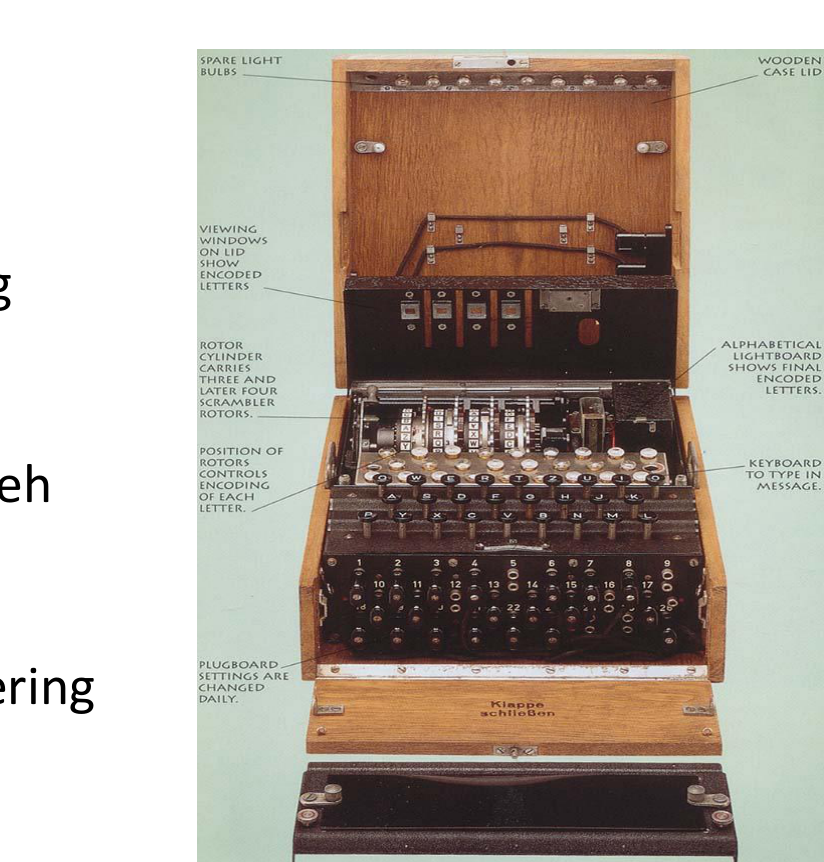
\includegraphics[width=90.09mm,height=237.01mm]{images/llm/page_057_img_01.png}%
\end{textblock*}

\newpage

% --- unit llm 58 ---
% === Halaman 58 (llm) ===

\section*{Tiga (3) Jenis Algoritma Kriptografi}

\subsection*{1. Algoritma kriptografi simetri (symmetric-key cryptography)}
\begin{itemize}
    \item Kunci enkripsi = kunci dekripsi, harus dijaga privat (rahasia) atau \textit{secret}
    \item Sudah ada sejak ribuan tahun yang hingga tahun 1976
\end{itemize}

\vspace{30mm}

\begin{itemize}
    \item Data Encryption Standard (DES)
    \item Advanced Encryption Standard (AES)
    \item Serpent
    \item Blowfish
    \item Loki
    \item MARS
    \item RC6
    \item Twofish
    \item 3-DES
    \item IDEA
    \item FEAL
    \item RC4
    \item SEAL
    \item Panama
    \item dll
\end{itemize}

% deskripsi: Diagram proses enkripsi dan dekripsi menggunakan kriptografi kunci simetri, menunjukkan input Plainteks P yang dienkripsi dengan Kunci privat K menjadi Cipherteks C, lalu didekripsi kembali dengan Kunci privat K menjadi Plainteks P.
% bbox normalisasi: [0.1600, 0.4500, 0.7600, 0.7100]
\begin{textblock*}{126.00mm}(33.60mm,133.65mm)
\noindent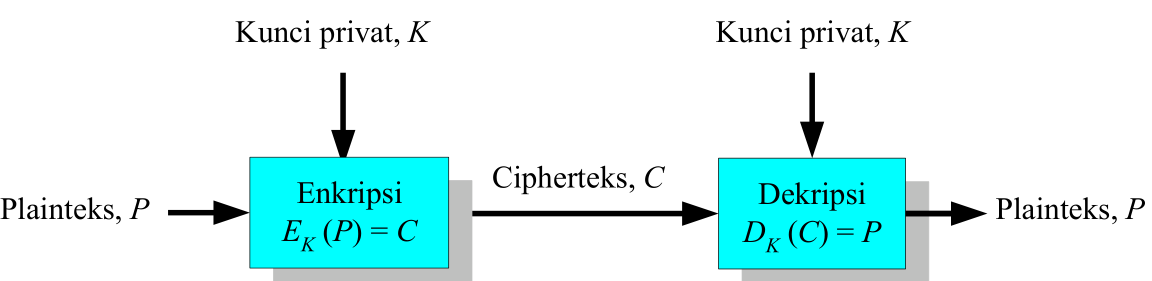
\includegraphics[width=126.00mm,height=77.22mm]{images/llm/page_058_img_01.png}%
\end{textblock*}

\newpage

% --- unit llm 59 ---
% === Halaman 59 (llm) ===

\vspace{196.02mm}

\textbf{Plaintext input}
\vspace{50mm}
\textbf{Ciphertext}
\vspace{50mm}
\textbf{Plaintext output}
\vspace{80mm}
Sumber: Cryptography in E-Commerce

% deskripsi: Diagram proses enkripsi dan dekripsi simetris yang menunjukkan penggunaan kunci yang sama (shared secret) untuk mengubah plaintext menjadi ciphertext dan kembali menjadi plaintext.
% bbox normalisasi: [0.1500, 0.1900, 0.7600, 0.8500]
\begin{textblock*}{128.10mm}(31.50mm,56.43mm)
\noindent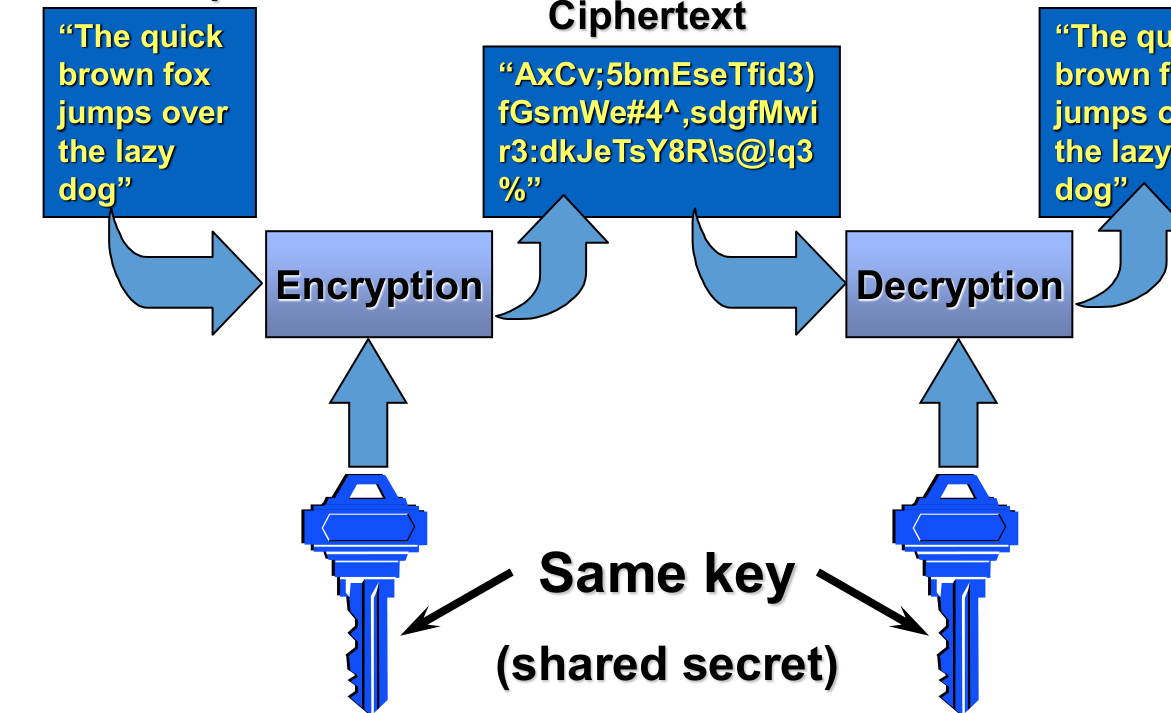
\includegraphics[width=128.10mm,height=196.02mm]{images/llm/page_059_img_01.png}%
\end{textblock*}

\newpage

% --- unit llm 60 ---
% === Halaman 60 (llm) ===

\section*{2. Algoritma kriptografi nir-simetri (asymmetric-key cryptography)}

\begin{itemize}
    \item Kunci enkripsi $\neq$ kunci dekripsi ($K1 \neq K2$)
    \begin{itemize}
        \item Kunci enkripsi $\rightarrow$ tidak rahasia (\textit{public key})
        \item Kunci dekripsi $\rightarrow$ rahasia (\textit{private key})
    \end{itemize}
    \item Mulai ditemukan sejak tahun 1976
\end{itemize}

\vspace{74.25mm}

\begin{flushright}
    \textcolor{red}{Nama lain: Kriptografi kunci--publik}\
    \textcolor{red}{(\textit{public-key cryptography})}
\end{flushright}

\vspace{20mm}

\begin{minipage}{0.45\textwidth}
    \begin{itemize}
        \item[--] RSA (Rivest-Shamir-Adleman)
        \item[--] ElGamal
        \item[--] DSA
        \item[--] Diffie-Hellman
        \item[--] Mercke Knapsack Algorithm
    \end{itemize}
\end{minipage}
\hfill
\begin{minipage}{0.45\textwidth}
    \begin{itemize}
        \item[--] Rabin
        \item[--] EPOC
        \item[--] Mc Eliece
        \item[--] XTR
        \item[--] ECC (\textit{Elliptic Curve Cryptography})
    \end{itemize}
\end{minipage}

% deskripsi: Diagram alur proses kriptografi kunci publik yang menunjukkan proses enkripsi menggunakan kunci publik K1 untuk mengubah Plainteks P menjadi Cipherteks C, dan proses dekripsi menggunakan kunci privat K2 untuk mengembalikan Cipherteks C menjadi Plainteks P.
% bbox normalisasi: [0.1600, 0.4500, 0.7800, 0.7000]
\begin{textblock*}{130.20mm}(33.60mm,133.65mm)
\noindent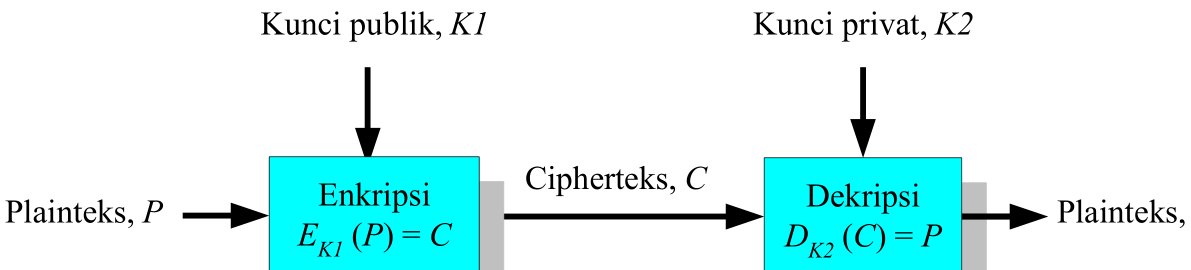
\includegraphics[width=130.20mm,height=74.25mm]{images/llm/page_060_img_01.png}%
\end{textblock*}

\newpage

% --- unit llm 61 ---
% === Halaman 61 (llm) ===

\vspace{210.87mm}

\textbf{Plaintext input}
\vspace{50mm}
\textbf{Public key} \quad \textbf{Different keys} \quad \textbf{Private key}
\vspace{20mm}
\textcolor{red}{Sumber: Cryptography in E-Commerce}

% deskripsi: Diagram alur enkripsi dan dekripsi asimetris yang menunjukkan proses perubahan plaintext input menjadi ciphertext menggunakan public key, dan pengembalian ciphertext menjadi plaintext output menggunakan private key.
% bbox normalisasi: [0.1200, 0.1500, 0.8300, 0.8600]
\begin{textblock*}{149.10mm}(25.20mm,44.55mm)
\noindent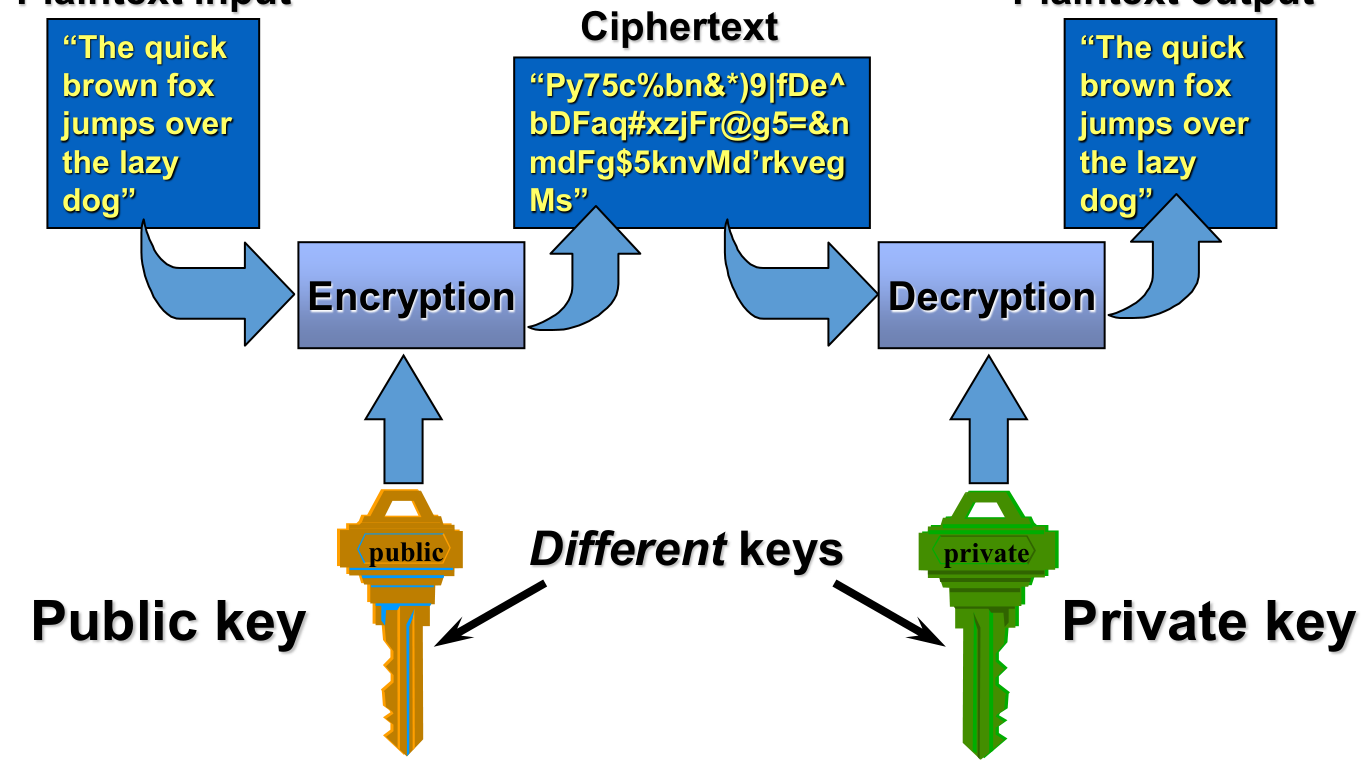
\includegraphics[width=149.10mm,height=210.87mm]{images/llm/page_061_img_01.png}%
\end{textblock*}

\newpage

% --- unit llm 62 ---
% === Halaman 62 (llm) ===

\section*{3. Fungsi Hash}

\begin{itemize}
    \item Mengkompresi pesan ukuran sembarang menjadi \textit{message-digest} berukuran \textit{fixed}.
    \item \textit{Irreversible} (tidak bisa dikembalikan menjadi pesan semula)
\end{itemize}

\vspace{10mm}

\begin{itemize}
    \item MD5
    \item SHA-1
    \item SHA-2
    \item Keccak (SHA-3)
    \item RIPEMD
    \item WHIRLPOOL
\end{itemize}

% deskripsi: Diagram alur fungsi hash yang menunjukkan input (Masukan) diproses oleh 'Fungsi hash' untuk menghasilkan 'Nilai hash' berupa string heksadesimal, dengan tiga contoh input yang berbeda.
% bbox normalisasi: [0.1200, 0.3800, 0.6300, 0.9200]
\begin{textblock*}{107.10mm}(25.20mm,112.86mm)
\noindent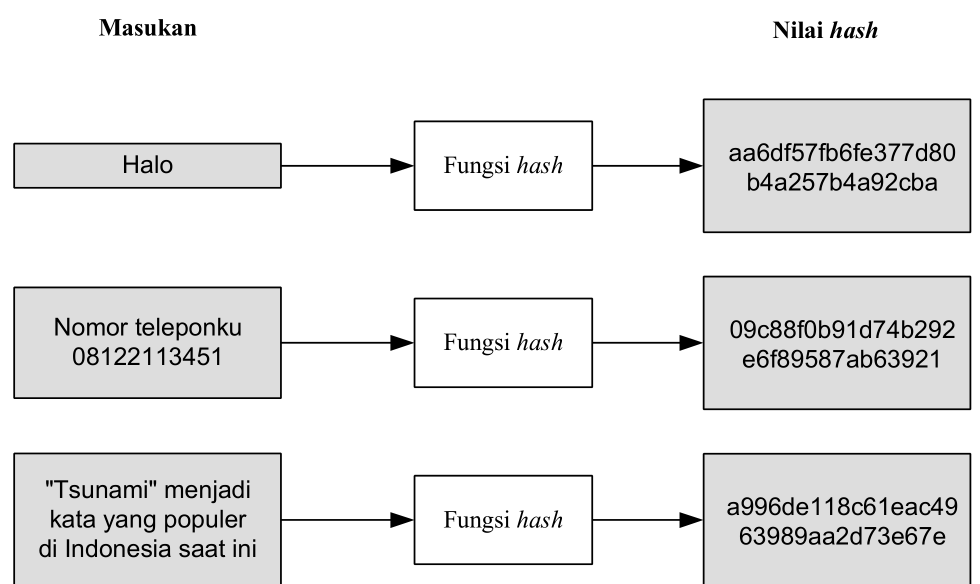
\includegraphics[width=107.10mm,height=160.38mm]{images/llm/page_062_img_01.png}%
\end{textblock*}

\newpage

% --- unit llm 63 ---
% === Halaman 63 (llm) ===

\vspace{163.94mm}

Kegunaan: memeriksa integritas pesan\vspace{10mm}

(Sumber gambar: Wikipedia)

% deskripsi: Diagram yang mengilustrasikan bagaimana perubahan kecil pada pesan input menghasilkan nilai hash kriptografis yang sangat berbeda, menunjukkan sensitivitas fungsi hash terhadap integritas pesan.
% bbox normalisasi: [0.1460, 0.2130, 0.7340, 0.7650]
\begin{textblock*}{123.48mm}(30.66mm,63.26mm)
\noindent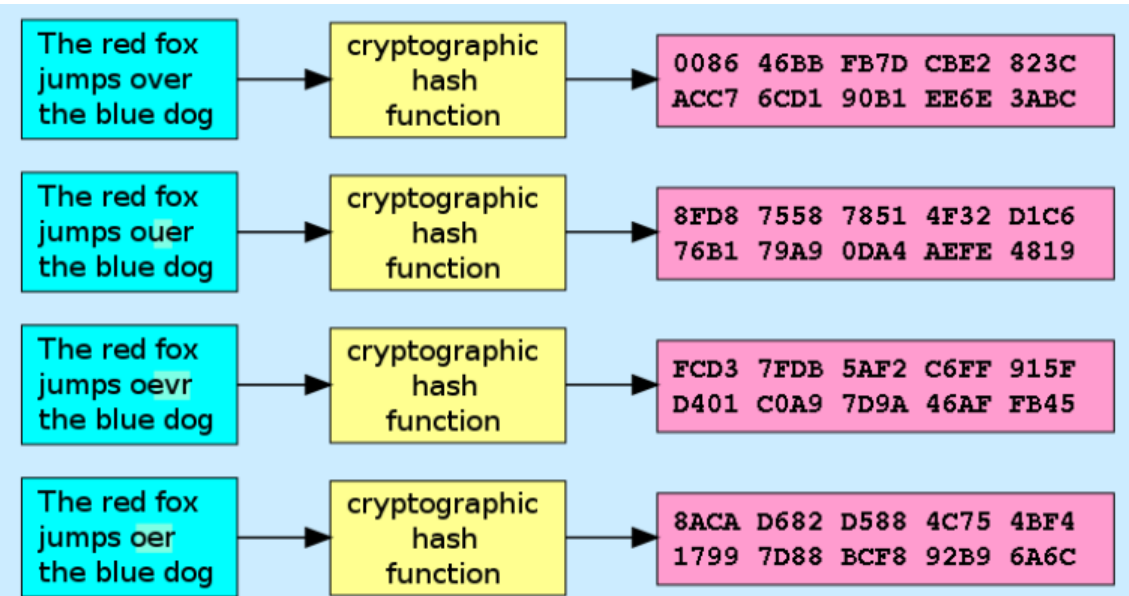
\includegraphics[width=123.48mm,height=163.94mm]{images/llm/page_063_img_01.png}%
\end{textblock*}

\newpage

% --- unit llm 64 ---
% === Halaman 64 (llm) ===

\section*{Lembaga Terkait Kriptografi di Indonesia}

\begin{enumerate}
    \item Badan Siber dan Sandi Negara (BSSN)\\
    \url{http://bssn.go.id}\\
    Merupakan penggabungan Lembaga Sandi Negara (Lemsaneg) dan Direktorat Jenderal Aplikasi Informatika (Aptika), Kementerian Komunikasi dan Informatika
    \vspace{10mm}
    \item Politeknik Siber dan Sandi Negara (PSSN)\\
    \url{https://poltekssn.ac.id/}
\end{enumerate}

\newpage

% --- unit llm 65 ---
% === Halaman 65 (llm) ===

\vspace{180.87mm}

Museum Sandi di Yogyakarta (Sumber: http://museum.lemsaneg.go.id/)

\vspace{80mm}

Alamat Jl. Faridan Muridan Noto No. 21, Kota Baru, Yogyakarta. Ini museum san satu-satunya di Indonesia, bahkan di dunia. Di dalamnya terdapat berbagai koleksi alat sandi yang pernah digunakan di Indonesia

% deskripsi: Foto bangunan Museum Sandi di Yogyakarta dengan arsitektur kolonial dan halaman depan yang luas.
% bbox normalisasi: [0.2210, 0.1560, 0.7620, 0.7650]
\begin{textblock*}{113.61mm}(46.41mm,46.33mm)
\noindent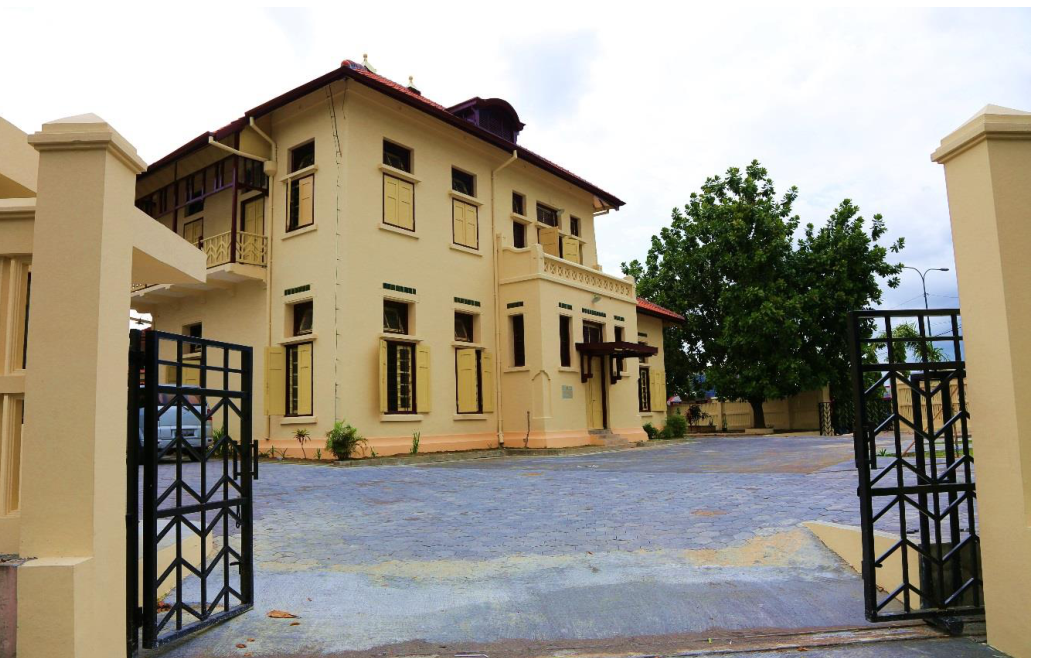
\includegraphics[width=113.61mm,height=180.87mm]{images/llm/page_065_img_01.png}%
\end{textblock*}

\newpage

% --- unit llm 66 ---
% === Halaman 66 (llm) ===

\vspace{218.00mm}

\begin{center}
\large Mesin sandi di Museum Sandi Yogyakarta
\end{center}

% deskripsi: Foto sebuah mesin sandi berwarna abu-abu dengan papan ketik (keyboard) dan panel kontrol, bertuliskan SN-101.
% bbox normalisasi: [0.2420, 0.0920, 0.7990, 0.8260]
\begin{textblock*}{116.97mm}(50.82mm,27.32mm)
\noindent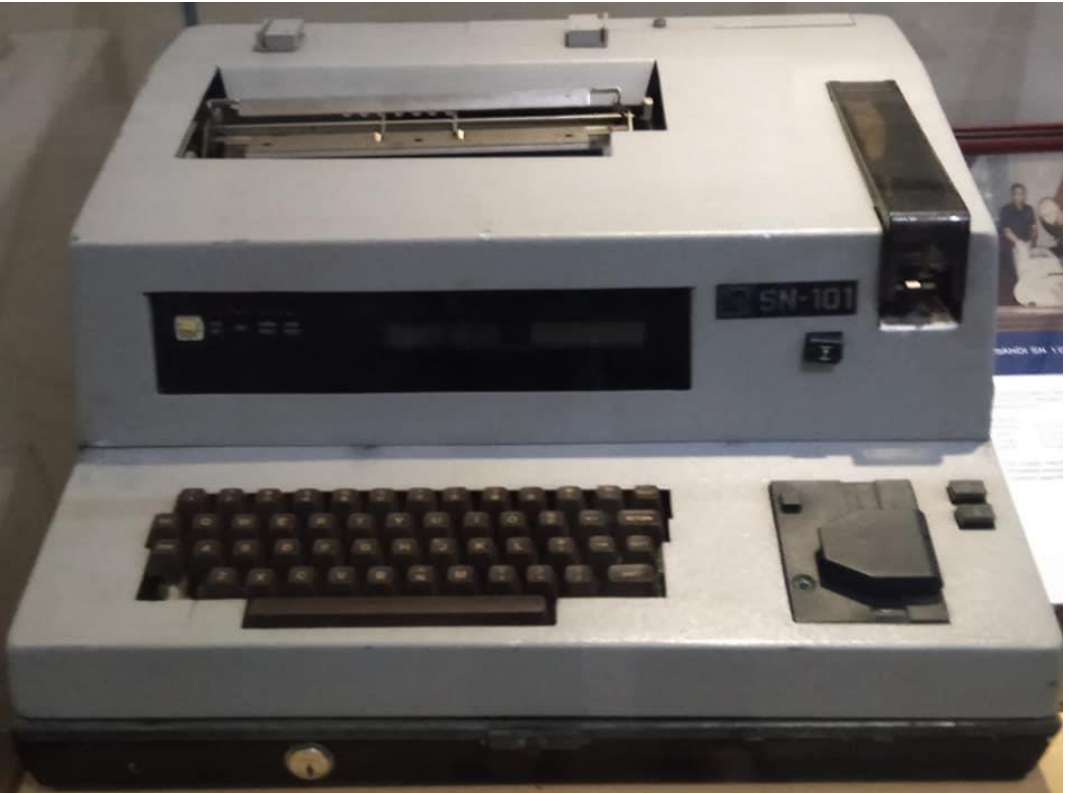
\includegraphics[width=116.97mm,height=218.00mm]{images/llm/page_066_img_01.png}%
\end{textblock*}

\newpage

% --- unit llm 67 ---
% === Halaman 67 (llm) ===

\section*{Tantangan Masa Depan Kriptografi}

\vspace{143.75mm}

\begin{itemize}
    \item Lightweight cryptography
\end{itemize}

\vspace{60mm}

Sumber: \url{https://www.researchgate.net/figure/Lightweight-cryptographic-primitives-for-IoT_fig9_338830634}

% deskripsi: Diagram hierarki Lightweight Cryptography Primitives yang terbagi menjadi Lightweight Block Ciphers, Lightweight Stream Ciphers, Lightweight Hash Functions, dan ECC.
% bbox normalisasi: [0.0900, 0.3660, 0.8820, 0.8500]
\begin{textblock*}{166.32mm}(18.90mm,108.70mm)
\noindent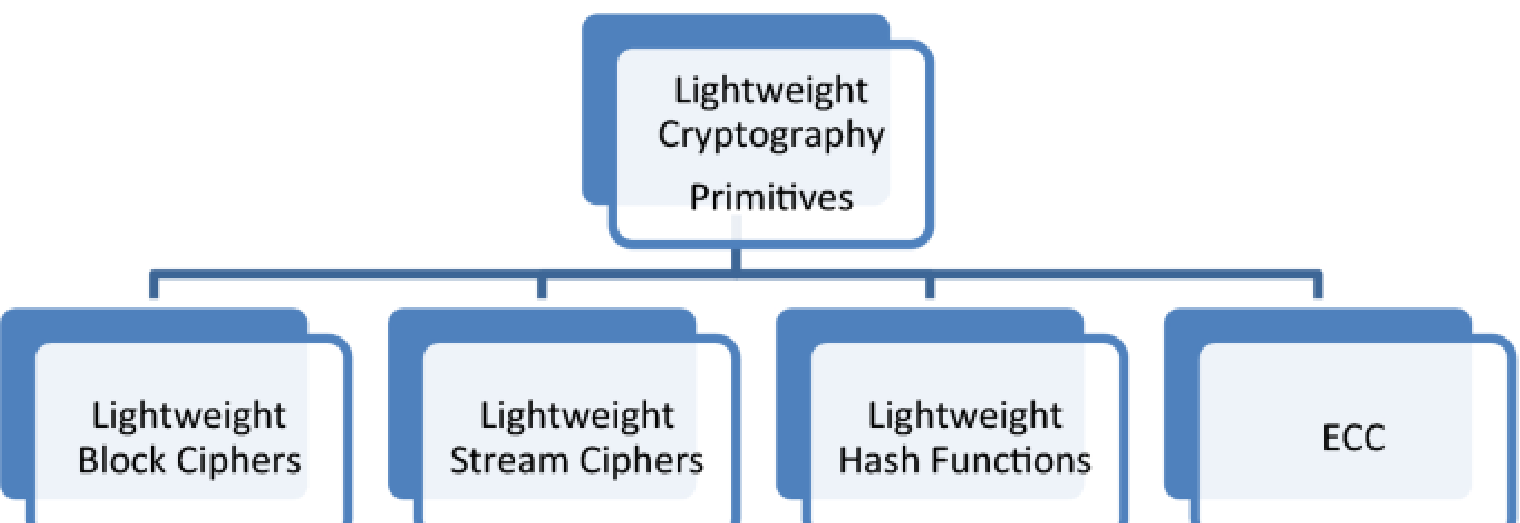
\includegraphics[width=166.32mm,height=143.75mm]{images/llm/page_067_img_01.png}%
\end{textblock*}

\newpage

% --- unit llm 68 ---
% === Halaman 68 (llm) ===

\begin{itemize}
  \item Post-quantum cryptography
\end{itemize}

\vspace{10mm}

\url{https://www.researchgate.net/figure/Basic-types-of-Post-Quantum-Cryptography-PQC_fig1_349071555}

% deskripsi: Diagram lingkaran yang menunjukkan empat tipe utama kriptografi pasca-kuantum (PQC): Hash-Based Signatures, Code-Based Cryptography, Multivariate Cryptography, dan Lattice-Based Cryptography.
% bbox normalisasi: [0.1530, 0.1820, 0.7600, 0.8340]
\begin{textblock*}{127.47mm}(32.13mm,54.05mm)
\noindent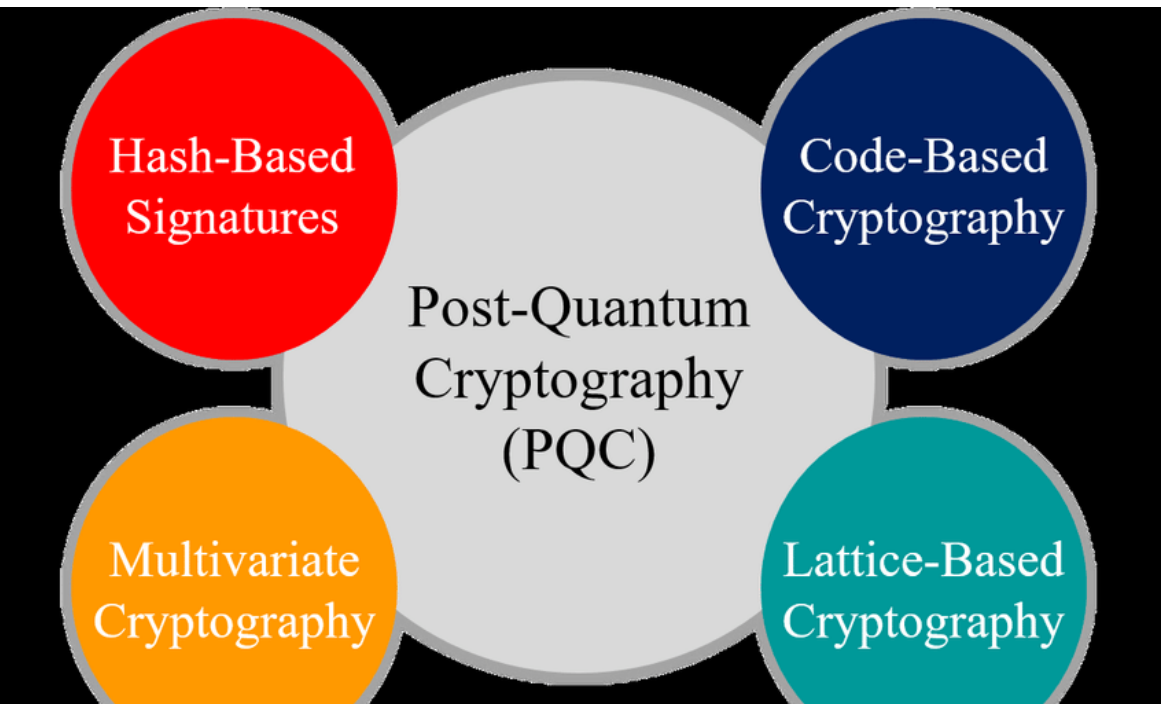
\includegraphics[width=127.47mm,height=193.64mm]{images/llm/page_068_img_01.png}%
\end{textblock*}

\newpage

% --- unit llm 69 ---
% === Halaman 69 (llm) ===

\begin{itemize}
  \item \textbf{Kriptografi berbasis AI dan serangan AI}
\end{itemize}

\vspace{10mm}

\url{https://www.linkedin.com/pulse/unlock-future-security-discover-how-ai-revolutionizing-cryptography-aelkc}

% deskripsi: Ilustrasi futuristik yang menunjukkan robot humanoid di atas platform digital dengan berbagai elemen keamanan siber seperti gembok digital dan jaringan data, dengan teks 'Unlock the Future of Security: Discover How AI is Revolutionizing Cryptography!'
% bbox normalisasi: [0.1220, 0.1700, 0.8410, 0.8960]
\begin{textblock*}{150.99mm}(25.62mm,50.49mm)
\noindent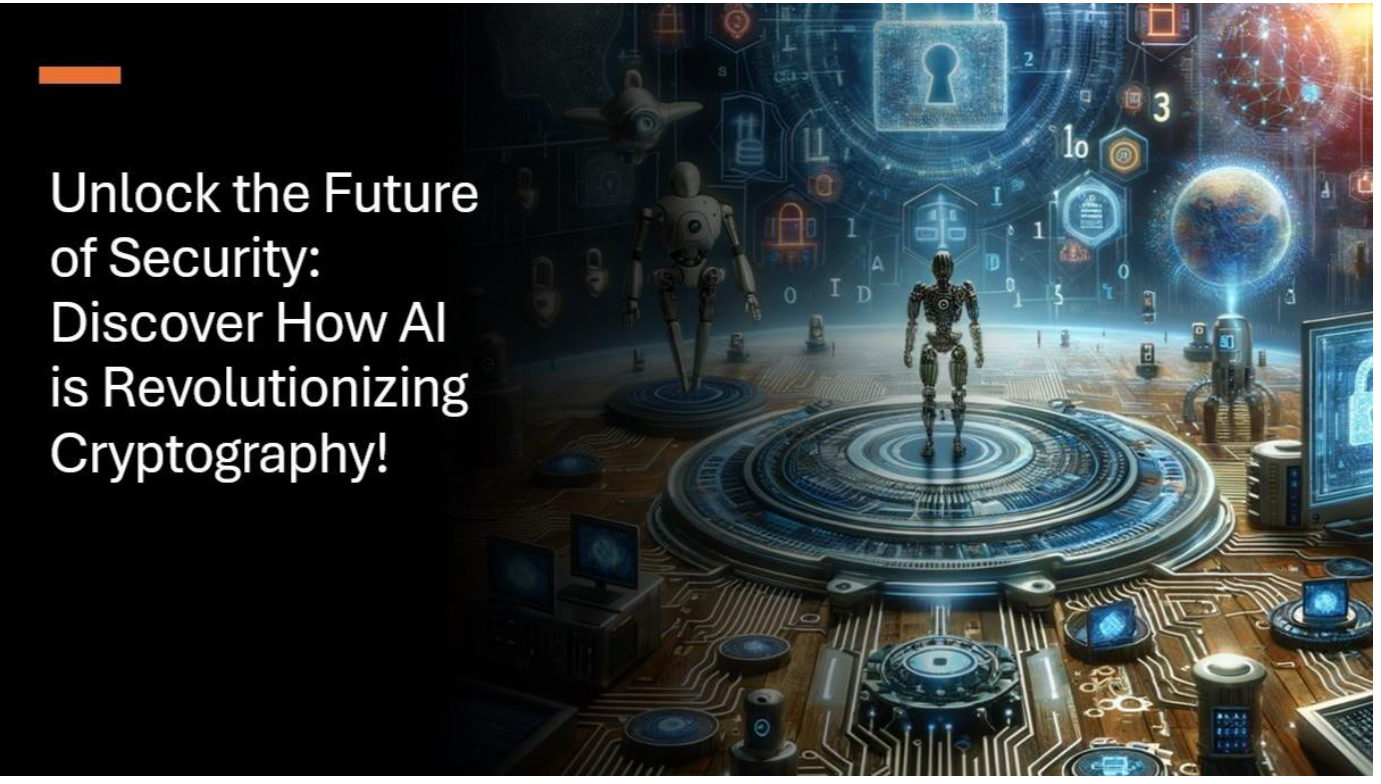
\includegraphics[width=150.99mm,height=215.62mm]{images/llm/page_069_img_01.png}%
\end{textblock*}

\newpage

% --- unit llm 70 ---
% === Halaman 70 (llm) ===

\section*{Selective encryption for multimedia data}

\vspace{60mm}

Sumber: \url{https://www.researchgate.net/figure/Selective-video-encryption-and-decryption-phases_fig3_353880117}

% deskripsi: Diagram alur proses Selective Video Encryption Phase dan Selective Video Decryption Phase yang menunjukkan tahapan mulai dari Key Generation, Selection Technique, hingga menjadi bitstream terenkripsi dan proses dekripsinya kembali menjadi gambar.
% bbox normalisasi: [0.1800, 0.2260, 0.7520, 0.8980]
\begin{textblock*}{120.12mm}(37.80mm,67.12mm)
\noindent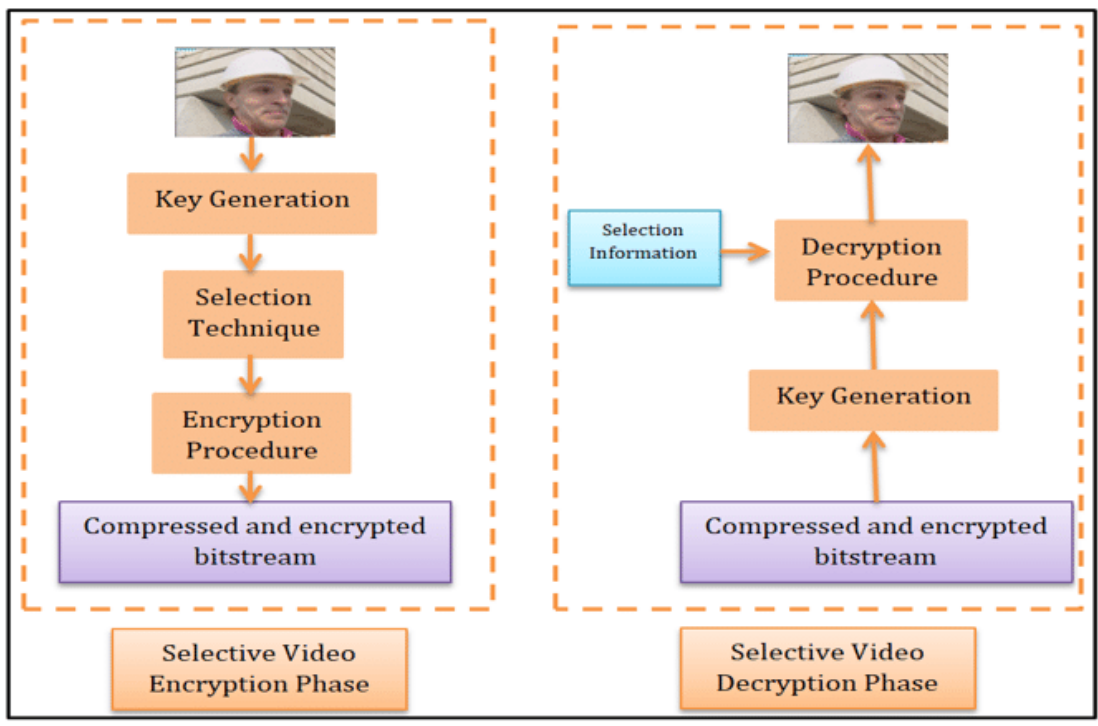
\includegraphics[width=120.12mm,height=199.58mm]{images/llm/page_070_img_01.png}%
\end{textblock*}

\newpage

% --- unit llm 71 ---
% === Halaman 71 (llm) ===

\section*{Beberapa kesalahan umum karena tidak paham kriptografi}

\vspace{187.11mm}

\begin{itemize}
    \item Menganggap enkripsi = encoding, hashing, tokenisasi.
    \item Tidak paham perbedaan \textit{symmetric encryption} dan \textit{asymmetric encryption}, kapan menggunakan \textit{symmetric} dan kapan menggunakan \textit{asymmetric encryption}
\end{itemize}

\vspace{10mm}

Sumber gambar: Slide kuliah tamu dari Burman Noviansyah

% deskripsi: Meme yang menunjukkan kebingungan antara enkripsi, hashing, dan Base64 menggunakan potongan gambar karakter film.
% bbox normalisasi: [0.6210, 0.2780, 0.9760, 0.9080]
\begin{textblock*}{74.55mm}(130.41mm,82.57mm)
\noindent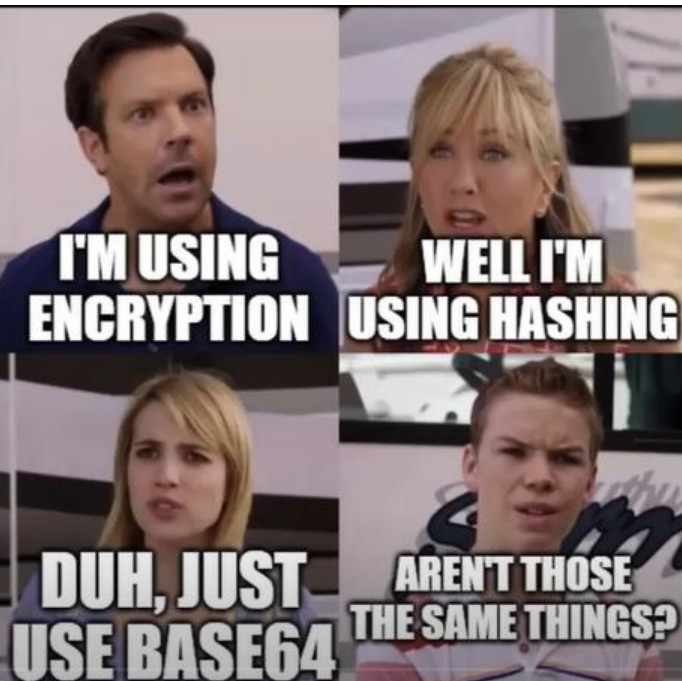
\includegraphics[width=74.55mm,height=187.11mm]{images/llm/page_071_img_01.png}%
\end{textblock*}

\newpage

% --- unit llm 72 ---
% === Halaman 72 (llm) ===

\begin{center}
\Huge \textcolor{yellow}{Encryption} Is Not \\
\Huge Encoding, Hashing, or Tokenization
\end{center}

\vspace{60mm}

\begin{center}
\fbox{\parbox{0.9\textwidth}{\textbf{Professional habit: define the exact protection goal before choosing the cryptographic primitive.}}}
\end{center}

\vspace{5mm}

Sumber gambar: Slide kuliah tamu dari Burman Noviansyah

% deskripsi: Infografis perbandingan antara Encoding, Hashing, Encryption, Tokenization, dan Signature yang mencakup definisi, contoh algoritma, dan tujuan utamanya.
% bbox normalisasi: [0.0900, 0.3500, 0.9100, 0.6100]
\begin{textblock*}{172.20mm}(18.90mm,103.95mm)
\noindent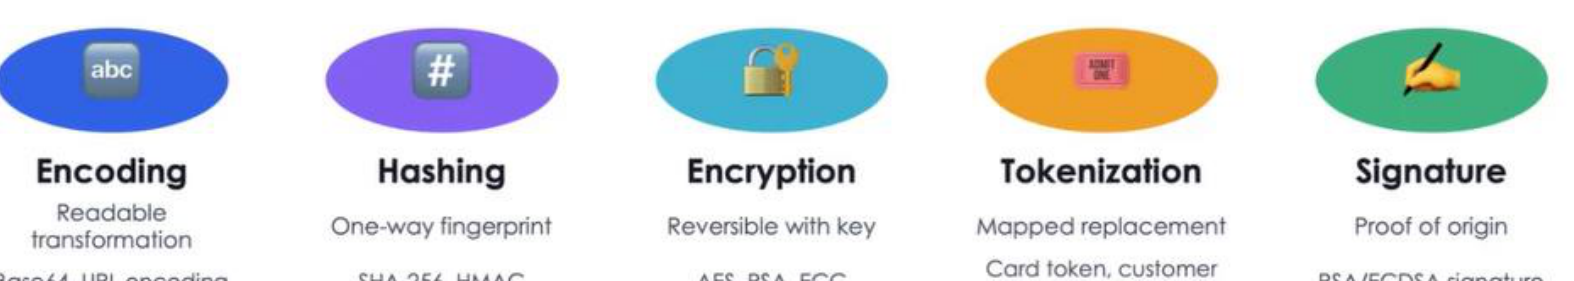
\includegraphics[width=172.20mm,height=77.22mm]{images/llm/page_072_img_01.png}%
\end{textblock*}

\newpage

% --- unit llm 73 ---
% === Halaman 73 (llm) ===

\begin{itemize}
    \item Tidak paham perbedaan \textit{symmetric encryption} dan \textit{asymmetric encryption}, kapan menggunakan \textit{symmetric/asymmetric encryption}
\end{itemize}

\end{document}
